


%!TEX TS-program = xelatex
%!TEX encoding = UTF-8 Unicode
%!BIB TS-program = biber
%!BIB program = biber
\documentclass[12pt,twoside]{book}
%\usepackage{extsizes}
\usepackage{geometry}                % See geometry.pdf to learn the layout options. There are lots.
\geometry{a4paper}                   % ... or a4paper or a5paper or ...
%\geometry{landscape}                % Activate for for rotated page geometry
%\usepackage[parfill]{parskip}    % Activate to begin paragraphs with an empty line rather than an indent section
\geometry{left=3cm}
\geometry{right=3cm}
\geometry{bottom=2cm}
\geometry{top=2cm}
\usepackage{graphicx}
\usepackage{amssymb}

\usepackage{polyglossia}
\usepackage[babel]{csquotes}
\setdefaultlanguage{german}

\usepackage{titlesec}
\usepackage{hyperref}
\usepackage[all]{hypcap} % Make references jump to the figure and not to the caption.
\usepackage{enumitem}

\usepackage{wasysym}
\usepackage{minted}

\usepackage{booktabs}
\usepackage{tabularx}

\usepackage{todonotes}

\usepackage{float}

\usepackage{tikz}

\usepackage{ifplatform}

\usepackage{savesym}
\savesymbol{iint}
\savesymbol{iiint}
\usepackage{amsmath}

\setlength{\parindent}{0cm}
\setlength{\parskip}{\medskipamount}

% Will Robertson's fontspec.sty can be used to simplify font choices.
% To experiment, open /Applications/Font Book to examine the fonts provided on Mac OS X,
% and change "Hoefler Text" to any of these choices.

\usepackage{fontspec,xltxtra,xunicode}

\ifmacosx
	\newcommand{\romanFont}{Linux Libertine O}
\else
	\newcommand{\romanFont}{Linux Libertine O}
\fi

\defaultfontfeatures{Mapping=tex-text}
\setmainfont[Mapping=tex-text]{\romanFont}
%\setsansfont[Scale=MatchLowercase,Mapping=tex-text]{Gill Sans}
%\setmonofont[Scale=MatchLowercase]{Andale Mono}
% \setmonofont[Mapping=tex-text,%
%     ItalicFont=Source Code Pro ExtraLight,%
%     BoldFont=Source Code Pro]{Source Code Pro Light}

%\newcommand{\HRule}{\rule{\linewidth}{0.1pt}}
%\newcommand{\logoheight}{2.5cm}

\renewcommand{\title}{Enterprise Infoboard - Intelligente Visualisierung und Austausch von heterogenen Informationen im Unternehmen}
\renewcommand{\author}{Tom Nick}
%\date{}                                           % Activate to display a given date or no date

% PDF properties
\hypersetup{
	pdftitle={\title{}},
	pdfauthor={\author{}}
}

\usepackage[style=numeric,natbib=true,backend=biber]{biblatex}
\bibliography{bachelorthesis}{}

\setlength{\bibitemsep}{8pt}
%\setlength{\bibhang}{0.2cm}

\usepackage{xpatch}
\xpretobibmacro{author}{\mkbibbold\bgroup}{}{}
\xapptobibmacro{author}{\egroup}{}{}
\xpretobibmacro{bbx:editor}{\mkbibbold\bgroup}{}{}
\xapptobibmacro{bbx:editor}{\egroup}{}{}

\renewcommand*{\labelnamepunct}{\mkbibbold{\addcolon\space}}


\usepackage{changepage}

\makeatletter
\renewcommand\listoffigures{%
    \section{\listfigurename}% Used to be \section*{\listfigurename}
      \@mkboth{\MakeUppercase\listfigurename}%
              {\MakeUppercase\listfigurename}%
    \@starttoc{lof}%
    }
\makeatother

\makeatletter
\renewcommand{\todo}[2][]{\tikzexternaldisable\@todo[#1]{#2}\tikzexternalenable}
\makeatother

\setcounter{secnumdepth}{3}
\setcounter{tocdepth}{2}

%\newcommand*{\fullref}[1]{\hyperref[{#1}]{\autoref*{#1} \nameref*{#1}}}
\newcommand*{\fullref}[1]{\hyperref[{#1}]{\autoref*{#1} (\nameref*{#1})}}

\newcommand{\makemu}{{\fontspec{Linux Libertine O}μ}}

\usepackage{multirow}

\usepackage{capt-of}

\usepackage[hang,flushmargin,bottom]{footmisc}

\newenvironment{absolutelynopagebreak}
  {\par\nobreak\vfil\penalty0\vfilneg
   \vtop\bgroup}
  {\par\xdef\tpd{\the\prevdepth}\egroup
   \prevdepth=\tpd}

\usepackage{titlesec}

\titleformat{\chapter}[display]
    {\normalfont\huge\bfseries}{\chaptertitlename\ \thechapter}{20pt}{\Huge}
\titlespacing*{\chapter}{0pt}{0pt}{40pt}

\usetikzlibrary{arrows,automata,positioning}

\usepackage{soul}

\usepackage{fancyhdr}
\fancyhead{}
\fancyfoot{}
\fancyhead[RE]{\textsc{\nouppercase{\rightmark}}}
\fancyhead[LO]{\textsc{\nouppercase{\leftmark}}}

\fancyfoot[CO,CE]{\thepage}
\pagestyle{fancy}

\setlength{\headheight}{14.5pt}

\let\cleardoublepage\clearpage

\usepackage[section]{placeins}

\usepackage{afterpage}
\newcommand\blankpage{%
    \null
    \thispagestyle{empty}%
    \addtocounter{page}{-1}%
    \newpage}

\usepackage{listings}



\begin{document}

% Titlepage
\begin{titlepage}
%\includegraphics[height=\logoheight,page=1]{Telekom_Logo_bw.pdf} \hfill \includegraphics[height=\logoheight,page=1]{TU_Logo.pdf}
\begin{center}
%\vspace{1cm}
%{\Huge Bachelor}\\
{\Huge \textsc{Technische Universität Berlin}}
{\fontsize{2.5cm}{2cm}\selectfont \textsc{Bachelor Thesis}\par}
\vspace{1cm}
\hrule
\vspace{0.3cm}
{\Huge \textsc{\title{}}\par}
~\\[0.1cm]
{\Large Supervisor: Prof. Dr. Dr. h.c. Albayrak}\\[0.1cm]
{\Large Advisors: Dipl.-Inform. Michael Meder}\\[0.3cm]
{\Large Written by \author{}}\\[0.1cm]
{\Large \today}
\vspace{0.55cm}
\hrule
\end{center}
%\vspace{1cm}
\vfill
\begin{center}{\Large\textbf{Abstract}}\end{center}

Das DAI-Labor ist eine der führenden Forschungseinrichtungen im Bereich verteilte Suchmaschinen - welche nun nicht mehr reine Forschung sind, sondern wie deren PIA-System von zahlreichen Verwaltungen als Alternative zu privaten Suchmaschinen benutzt wird. Ein interessantes Problem bei Suchmaschinen mit komplett separaten Suchindizes ist es die Ergebnisse dieser zusammen zu führen und dem Endbenutzer zu visualisieren. Diese Arbeit zielt darauf ab eine Visualisierungsform die ähnlich zu einer \textit{Social Media Wall} sein soll, für diese Ergebnisse zu untersuchen und zu erstellen.
Ein weiteres Themengebiet des DAI-Labors ist die Gamification im Enterprise Bereich, so werden auch diese Mechanismen untersucht und benutzt, um die Benutzung der Applikation zu fördern.
Außerdem wird ausführlich auf die neuen Entwicklungsmethoden im Bereich der Webapplikationen eingegangen und aufgezeigt, wie diese die Entwicklung vereinfachen und verbessern können.
Das Ergebnis dieser Arbeit ist eine voll funktionsfähige und mit neuesten Methoden entwickelte Webapplikation, die ein innovatives Interface für Suchergebnisse besitzt und deren Benutzung durch nahtlos eingebundene Spielelemente gefördert wird.

\end{titlepage}

\pagenumbering{roman}

%\blankpage

\chapter*{Declaration of authorship}

I hereby certify that the thesis I am submitting is entirely my own original work except where otherwise indicated. I am aware of the University's regulations concerning plagiarism, including those regulations concerning disciplinary actions that may result from plagiarism. Any use of the works of any other author, in any form, is properly acknowledged at their point of use.\footnote{The template for this declaration of authorship was taken from \url{https://www.wiwi.hu-berlin.de/international/mems/upload/authorship}.}

\vspace{2cm}

Berlin, \today\\
\textbf{Place, date}\hfill\textbf{Signature}

\tableofcontents
\newpage

\pagenumbering{arabic}

\chapter{Einleitung}

Die gemeinsame Darstellung von Inhalten aus verschiedenen Quellen ist ein interessantes und weit erforschtes Thema. Die grundsätzliche Idee ist es, dem Benutzer die Benutzung bzw. die Konsumierung von Inhalten angenehmer und effizienter zu gestalten, indem ein einheitliches Interface für Inhalte geschaffen wird. Vor der \textit{digitalen Revolution} war das ein äußerst aufwendiges und kostspieliges Unterfangen, als Beispiel seien die frühen Enzyklopädien genannt, da diese versuchen, sämtliches Wissen an einem Ort in homogener Sprache und Darstellung bereitzustellen. Durch die momentan verfügbaren Technologien ist das Erstellen einer einheitlichen Datenquelle für verschiedene Inhalte deutlich einfacher geworden, wobei die Schwierigkeit einer guten Zusammenführung dennoch weiterhin besteht und Produkte, die das gut lösen, sehr erfolgreich sind - wie z.B. die Aggregation sozialer Aktivitäten bei Facebook.
Wenn man sich jedoch auf eine Teilmenge der verfügbaren Informationen beschränkt, wie Nachrichten die per RSS verfügbar sind, ist es deutlich einfacher eine angemessene Zusammenstellung der Inhalte zu gestalten. Prominentes Beispiel für eine Anwendung dieser Art ist die Nachrichten-Applikation pulse \cite{pulse}, die auf Basis von RSS ein angenehmes und attraktives Interface für die gleichzeitige Konsumierung mehrerer Nachrichtenseiten anbietet. Der Erfolg von \textit{pulse} spricht für sich mit ca. 22 Millionen Downloads auf dem Android-System.
Eine der komplexesten Zusammenführungen von Informationen unterschiedlichster Art stellen Suchmaschinen da, da hier eine Reduzierung der benutzten Informationen, eine sofortige Verschlechterung der Suchergebnisse bewirkt - die ideale Suchmaschine würde jede mögliche Datenquelle und jedes existierende Dateiformat indizieren.
Suchmaschinen der jetzigen Zeit versuchen sich diesem Optimum immer weiter zu nähern und können mittlerweile eine Vielzahl an Datenformaten und Datenquellen benutzen.
Trotz der unendlichen Diversität der indizierten Daten werden die Suchergebnisse meistens über eine einfache Auflistung in Textform dargestellt, weil jedes Dateiformat mehr oder minder auf Text reduziert werden kann.
Neue Visualisierungsformen für Suchergebnisse sind überraschenderweise bisher wenig untersucht worden, andere Bereiche waren da experimentierfreudiger, wie z.B. die Zusammenführung von Social-Media-Kanälen mithilfe von \textit{Social Media Walls}.
Sie sind eine Form der Darstellung für Inhalte mit kurzen Texten und Bildern aus verschiedenen sozialen Kanälen. Die Besonderheit liegt in der Homogenisierung der Inhalte und in der gleichzeitigen Darstellung von verschiedenen Kanälen.
Suchergebnisse besitzen ganz ähnliche Attribute wie die Datenpunkte von Social-Media-Kanälen, womit die Frage nahe liegt, ob die Visualisierung von Suchergebnissen verbessert werden kann, indem eine ähnliche Darstellung wie der von \textit{Social Media Walls} benutzt wird.
Diese Arbeit bemüht sich diese Frage zu beantworten und eine neue Visualisierungsform für Suchergebnisse zu finden mit der Inspiration von \textit{Social Medial Walls}.

Der Einsatz von Gamification hat in den letzten Jahren stetig zugenommen, da es ein äußerst effektives Mittel ist, um das Erlebnis des Nutzers zu erhöhen und dadurch seine Interaktionen mit der Seite zu fördern.
Die Benutzung von Gamification im Enterprise-Bereich bzw. in kleinen sozialen Kreisen ist jedoch bisher noch nicht allzu populär. Die prominentesten Beispiele sind Sport-Apps, bei denen Freunde sich miteinander vergleichen können, wie Strava \cite{strava} oder Nike+ \cite{nike}. Eine Integration stellt damit in diesem Bereich eine interessante Herausforderung dar, dessen Potential bisher noch nicht vollständig geklärt ist.


\section{Anforderungen}

Die Anforderungen an die Applikation waren anfangs größtenteils noch offen. Die genauen Spezifikationen haben sich während der Ausarbeitung ergeben.

\begin{description}

\item[Darstellung von Daten]

Einer der Hauptanforderungen ist die Darstellung von Suchergebnissen (im zukünftigen Verlauf des Textes wird sie als Kacheln bezeichnet) im Stil einer \textit{Social Media Wall}. Daraus folgen weitere Anforderungen, z.B. dass es unterschiedliche Kacheln gibt - also für verschiedene Daten verschiedene Darstellungen. Es könnten auch Suchergebnisse für Kontakte und Webseiten ganz unterschiedlich aufgebaut sein. Die dargestellten Inhalte sind weiterhin dynamisch, während des Betriebes können Kacheln hinzukommen, entfernt oder anderen Suchbegriffen zugeordnet werden. Die Kacheln bieten zudem Interaktionsmöglichkeiten, sie können bewertet und favorisiert werden.

\item[Bewertungssystem]

  Der Benutzer soll in der Lage sein, angezeigte Suchergebnisse zu bewerten und dadurch die Priorisierung von Suchergebnissen zukünftiger Anfragen für \textbf{alle} Benutzer zu verändern.

\item[Benutzung mehrerer Datenquellen]
  Die angezeigten Suchergebnisse können aus mehreren Datenquellen kommen, d.h. die gleichzeitige Darstellung von Suchergebnissen von z.B. Facebook mit denen von Twitter. Hier war es wieder besonders wichtig, dass man einfach neue Datenquellen hinzufügen kann.

\item[Authentifizierungssystem]
	Zur Benutzung der Gamification-Elemente und der Suchanfrage bedarf es einer Authentifizierung. Es muss sichergestellt werden, dass kein Benutzer der nicht authentifiziert ist, Zugriff auf die Applikation hat.

\item[Single Page Application]
  Es soll eine sogenannte \textit{Single Page Application} erstellt werden, d.h. eine Webapplikation bei der JavaScript abseits des initialen Seitenaufrufes alles rendert. Im Gegensatz zur klassischen Methodik bei der jede Interaktion in einer komplett neuen Seite, die vom Server gerendert wird, resultiert.

\item[Gamification]
  Um die Benutzung der Seite zu animieren sollen Gamification-Methoden eingeführt werden wie z.B. Punkte für das tägliche einloggen bis hinzu erweiterten Methoden wie der Erstellung eines Compulsion Loop.

\item[Konfiguration]
  Es muss möglich sein viele Parameter anzupassen, einige davon auch als Benutzerinterface für den Benutzer andere wiederum als simple Konfigurationsdatei für verwendete URLs und ähnliches.

\end{description}

\section{Relevante Arbeiten}

Da die Applikation mehrere Gebiete vereint als etwas bestehendes weiterzuentwickeln, gibt es direkt keine relevanten Arbeiten. Jedoch ist es nützlich bestehendes in den einzelnen Gebieten zu untersuchen.

\subsection{Social Media Walls}

Eine sehr gute Auflistung verschiedener \textit{Social Media Wall}-Applikationen bietet \citep{hofram}. Die Homogenität dieser Angebote ist erstaunlich, würde man die Produkte zweier verschiedener Anbieter nebeneinander sehen, wären die größten Unterschiede stilistischer Natur wie benutzte Farben und Schriftarten. Leider sind die wenigsten Produkte in einer Demo zu testen, da die Lösungen üblicherweise auf den Kunden zugeschnitten werden. Der Verwendungszweck mit dem am meisten geworben wird sind große Veranstaltungen wie Konzerte, weswegen auch keine im Produktiveinsatz eingesehen werden konnten. In \ref{fig:socialwall} kann eine der Implementierungen gesehen werden.\\

\begin{figure}[H]
    \centering
    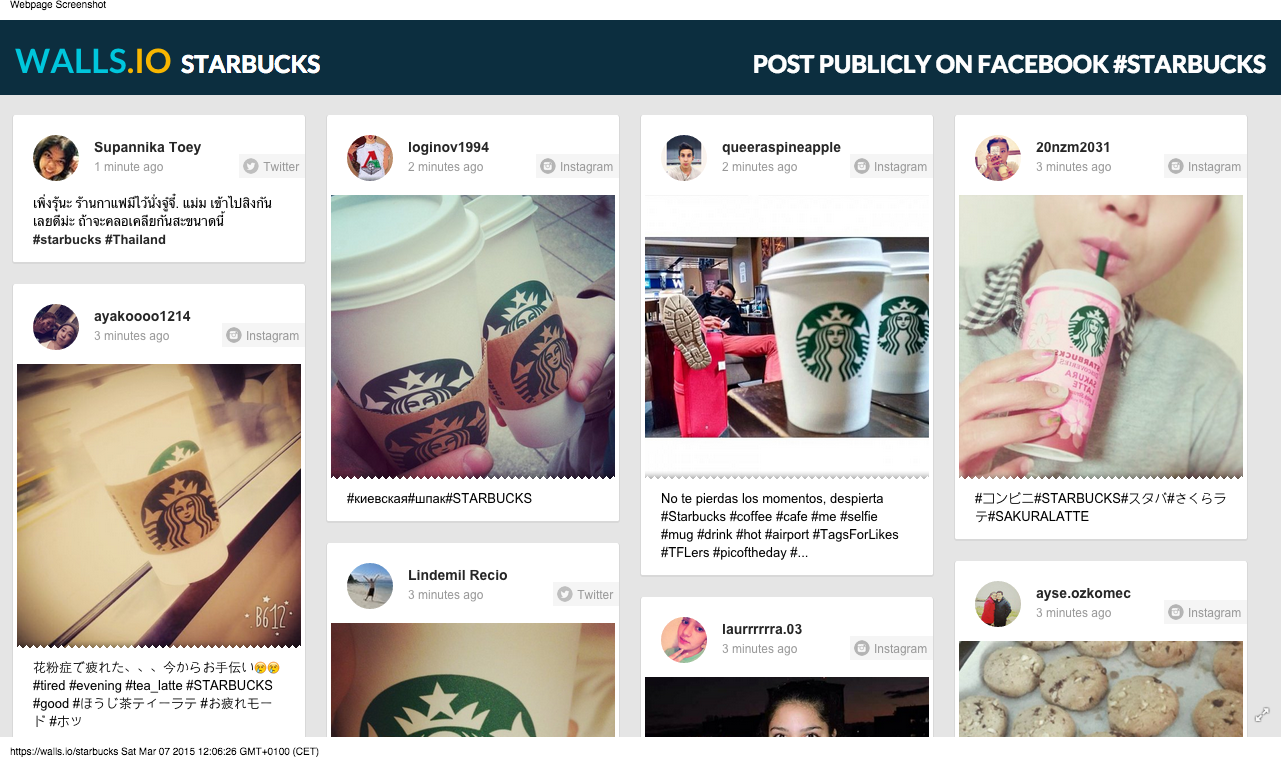
\includegraphics[width=0.8\textwidth]{images/Starbucks.png}
    \caption{Eine \textit{Social Media Wall} vom Anbieter walls.io \cite{wallsio}}
    \label{fig:socialwall}
\end{figure}

Insofern sind diese Angebote für diese Arbeit nicht wirklich lohnenswert weiter zu analysieren und werden als grobe Inspiration für das Design benutzt.

\subsection {Gamification}

Es gibt einige gute Beispiele von Seiten die ähnliche Inhalte anzeigen und erfolgreich Gamification implementiert haben. Einen schwachen aber effektiven Ansatz verfolgt die Social-News-Seite reddit \cite{reddit}. Jegliche Inhalte (eingereichte Links, Kommentare) der Seite können binär bewertet werden (im reddit-jargon wird hier von \textit{upvotes} und \textit{downvotes} gesprochen). Reicht man nun selbst etwas ein und andere Benutzer bewerten den eingereichten Inhalt, wird die Differenz aus \textit{upvotes} und \textit{downvotes} einem als Karma gutgeschrieben. Karma besitzt ähnlich wie die in Videospielen erreichte Punktzahl keinen Wert in dem Sinne, dass mit ihr nichts weiter gemacht werden kann als den Wert mit den von anderen zu vergleichen.
Dieser Gamification-Aspekt ist ein nicht zu unterschätzender Teil von reddit bzw. dem Erfolg von reddit welcher beachtlich ist, laut Alexa ist reddit die 32 meist besuchte Webseite der Welt, in den USA ist sie sogar Platz 10 \cite{alexa}.
Eine ausführliche Untersuchung von \citep{richerichkarma} zeigt die Tragweite von reddits Karma-System. Es dient demnach vor dienlich als Bewertung des eingereichten Inhalts durch andere bzw. die daraus resultierende Selbstbestätigung wenn das eigene Karma erhöht wird.
Benutzer reddits werden dadurch jedoch darauf gepolt ihre eingereichten Beiträge nach der Anzahl an Karma, welches der Beitrag liefern wird, auszusuchen.

DAIKnow \citep{meder2014daiknow} ist eine Bookmarking Seite ähnlich zu delicous.com\cite{delicious} bei der Links mit Beschreibungen und Keywords eingereicht werden können. Durch den gezielten Einsatz von Punkten, Abzeichen und Bestenlisten wird die Benutzung der Seite durch die Benutzer gesteigert. Im Gegensatz zu reddit ist dieses System jedoch weitaus komplexer, so bekommt man z.B. Punkte für den täglichen Aufruf, Punkte für das Einrechen eines Links oder das jemand anderes seinen Link kopiert hat.
Ein Problem das sich auftat bei DAIKnow war dass häufige Benutzer alle verfügbaren Abzeichen freischalteten und damit der Gamification-Aspekt damit kein Grund mehr ist die Applikation weiter zu benutzen.

\chapter{Konzeptuelle Umsetzung}\label{chap:concept}

Einer der wichtigsten Aspekte einen Interface-getriebene Applikation ist das Nutzererlebnis, in diesem Kapitel werden die zwei wichtigsten Punkte dieser Arbeit die für das Nutzererlebnis wichtig sind, vornehmlich Gamification und die Visualisierung der Suchergebnisse analysiert und ein Konzept wird ausgearbeitet welches schlussendlich in \ref{chap:tech} umgesetzt wird.

\section{Visualisierung der Suchergebnisse}\label{chap:concept:wall}

Heutige Webtechnologien erlauben nahezu uneingeschränkte Möglichkeiten Daten zu visualisieren, abseits von der initialen Idee eine Darstellung ähnlich einer \textit{Social Media Wall} zu benutzen gibt es eine viel zahl an Parametern betrachtet werden müssen - vornehmlich jedoch Layout, Animationen und das Design der individuellen Suchergebnisse.

\subsection{Layout}

Wie Pinterest\cite{pinterest} oder das Metro-Design von Microsoft gezeigt haben ist aktuell eine der besten Darstellung für Medieninhalte verschiedener Art ein Layout basierend auf Kacheln, siehe \ref{fig:metro_pinterest}.

\begin{figure}[H]
    \centering
    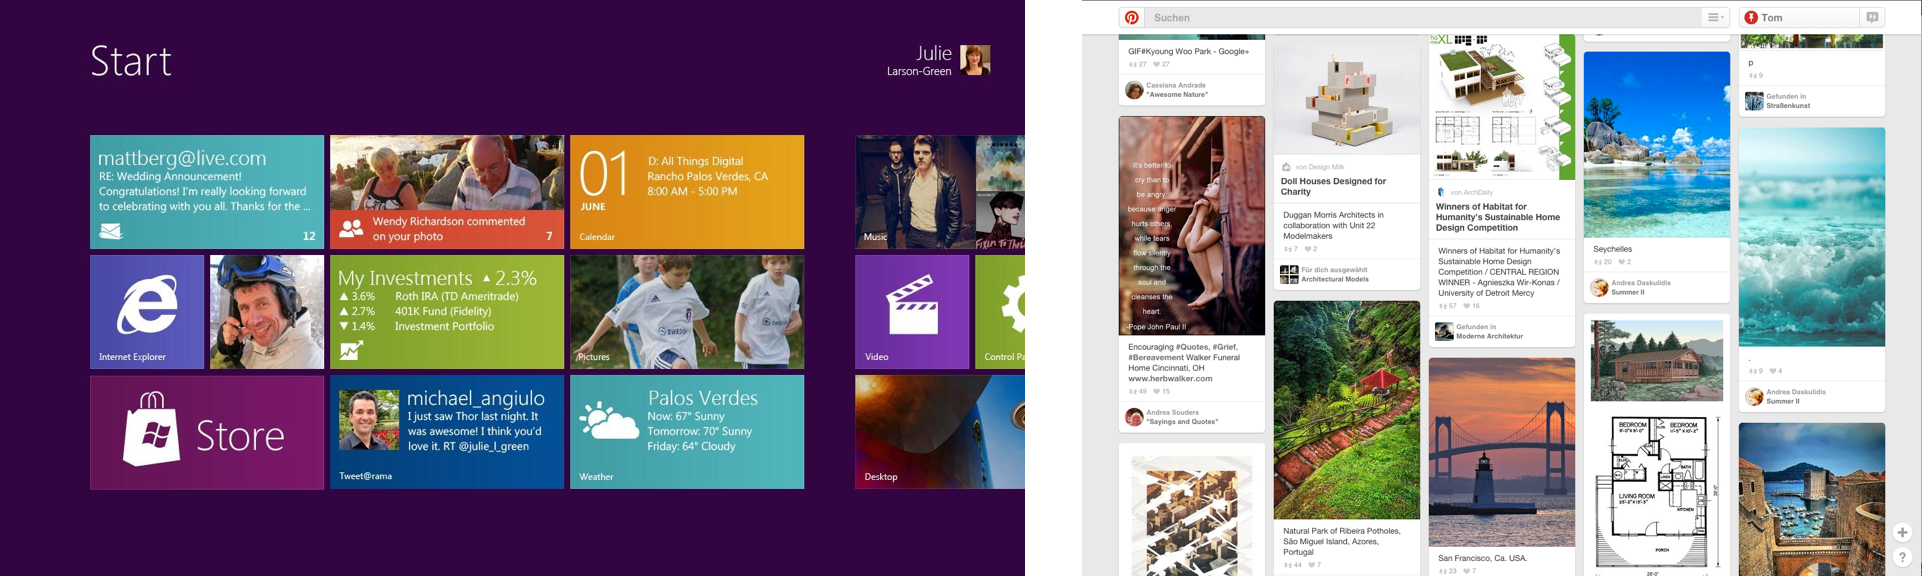
\includegraphics[width=0.8\textwidth]{images/metro_pinterest.png}
    \caption{Links das Rasterbasierte Layout von Windows 8, rechts das Spaltenbasierte Layout von Pinterest. Das Linke Bild ist genommen von \cite{metrodesign}}
    \label{fig:metro_pinterest}
  \end{figure}

Es gibt oft eine Regel nach welchem Muster die Kacheln angeordnet werden sollen, z.B. sollten die neuesten Kacheln an oberster Stelle gezeigt werden oder \textit{wichtigere} Kacheln prominenter dargestellt werden. Die Kacheln für das Infoboard unterliegen der Regel das sie anhand ihrer Wertung angeordnet werden müssen. Die folgende Analyse wird deshalb viel Wert darauf legen wie sich das Layout verhält, wenn neue Kacheln hinzukommen und damit neu sortiert werden müssen.
Im folgenden wird die Rasterbasierte mit der Spaltenbasierten Darstellung der Kacheln verglichen, da diese populäre Darstellungen in diesem Bereich sind, die erfolgreich verwendet wurden.

\begin{itemize}
  \item \textbf{Spaltenbasierte Anordnung} \\
  Bei dieser Form werden die einzelnen Kacheln mit einheitlicher Breite und variabler Höhe in Spalten in der Größenordnung von 3-5 dargestellt.

  \begin{figure}[H]
    \centering
    \includegraphics[width=0.5\textwidth]{images/livewall_columns.pdf}
    \caption{Spaltenbasierte Anordnung der Inhalte}
    \label{fig:awesome_image}
  \end{figure}

  \textbf{Vorteile} \\
  Die Vorteile liegen in der Simplizität der Implementierung und der Intuitivität des Inhalt-Flusses d.h. neuer Inhalt wird oben eingefügt und alter rutscht nach unten, wobei jeweils nur eine Spalte \textit{verrutscht} je neu eingefügter Kachel.
  Weiterhin ermöglicht die Variable Höhe viel Flexibilität bei dem Anzeigen des Inhalts - z.B. können lange Texte angemessen gut angezeigt werden ohne die Zeichenanzahl zu begrenzen oder ähnliche Limitierungen einzuführen.

  \textbf{Nachteile}\\
  Der größte Nachteil ist die Starrheit des Layouts, da alle Objekte die gleiche Breite haben ist man stark limitiert wie man die Inhalte darstellt. Abstriche müssen auch gemacht werden bei der Sortierung der Inhalte: Sobald die angezeigten Kacheln einer Sortierung unterliegen, kann der Inhaltsfluss nicht optimal funktionieren, siehe \ref{fig:livewall_sort} für eine visuelle Erklärung.
  
  \begin{figure}[H]
    \centering
    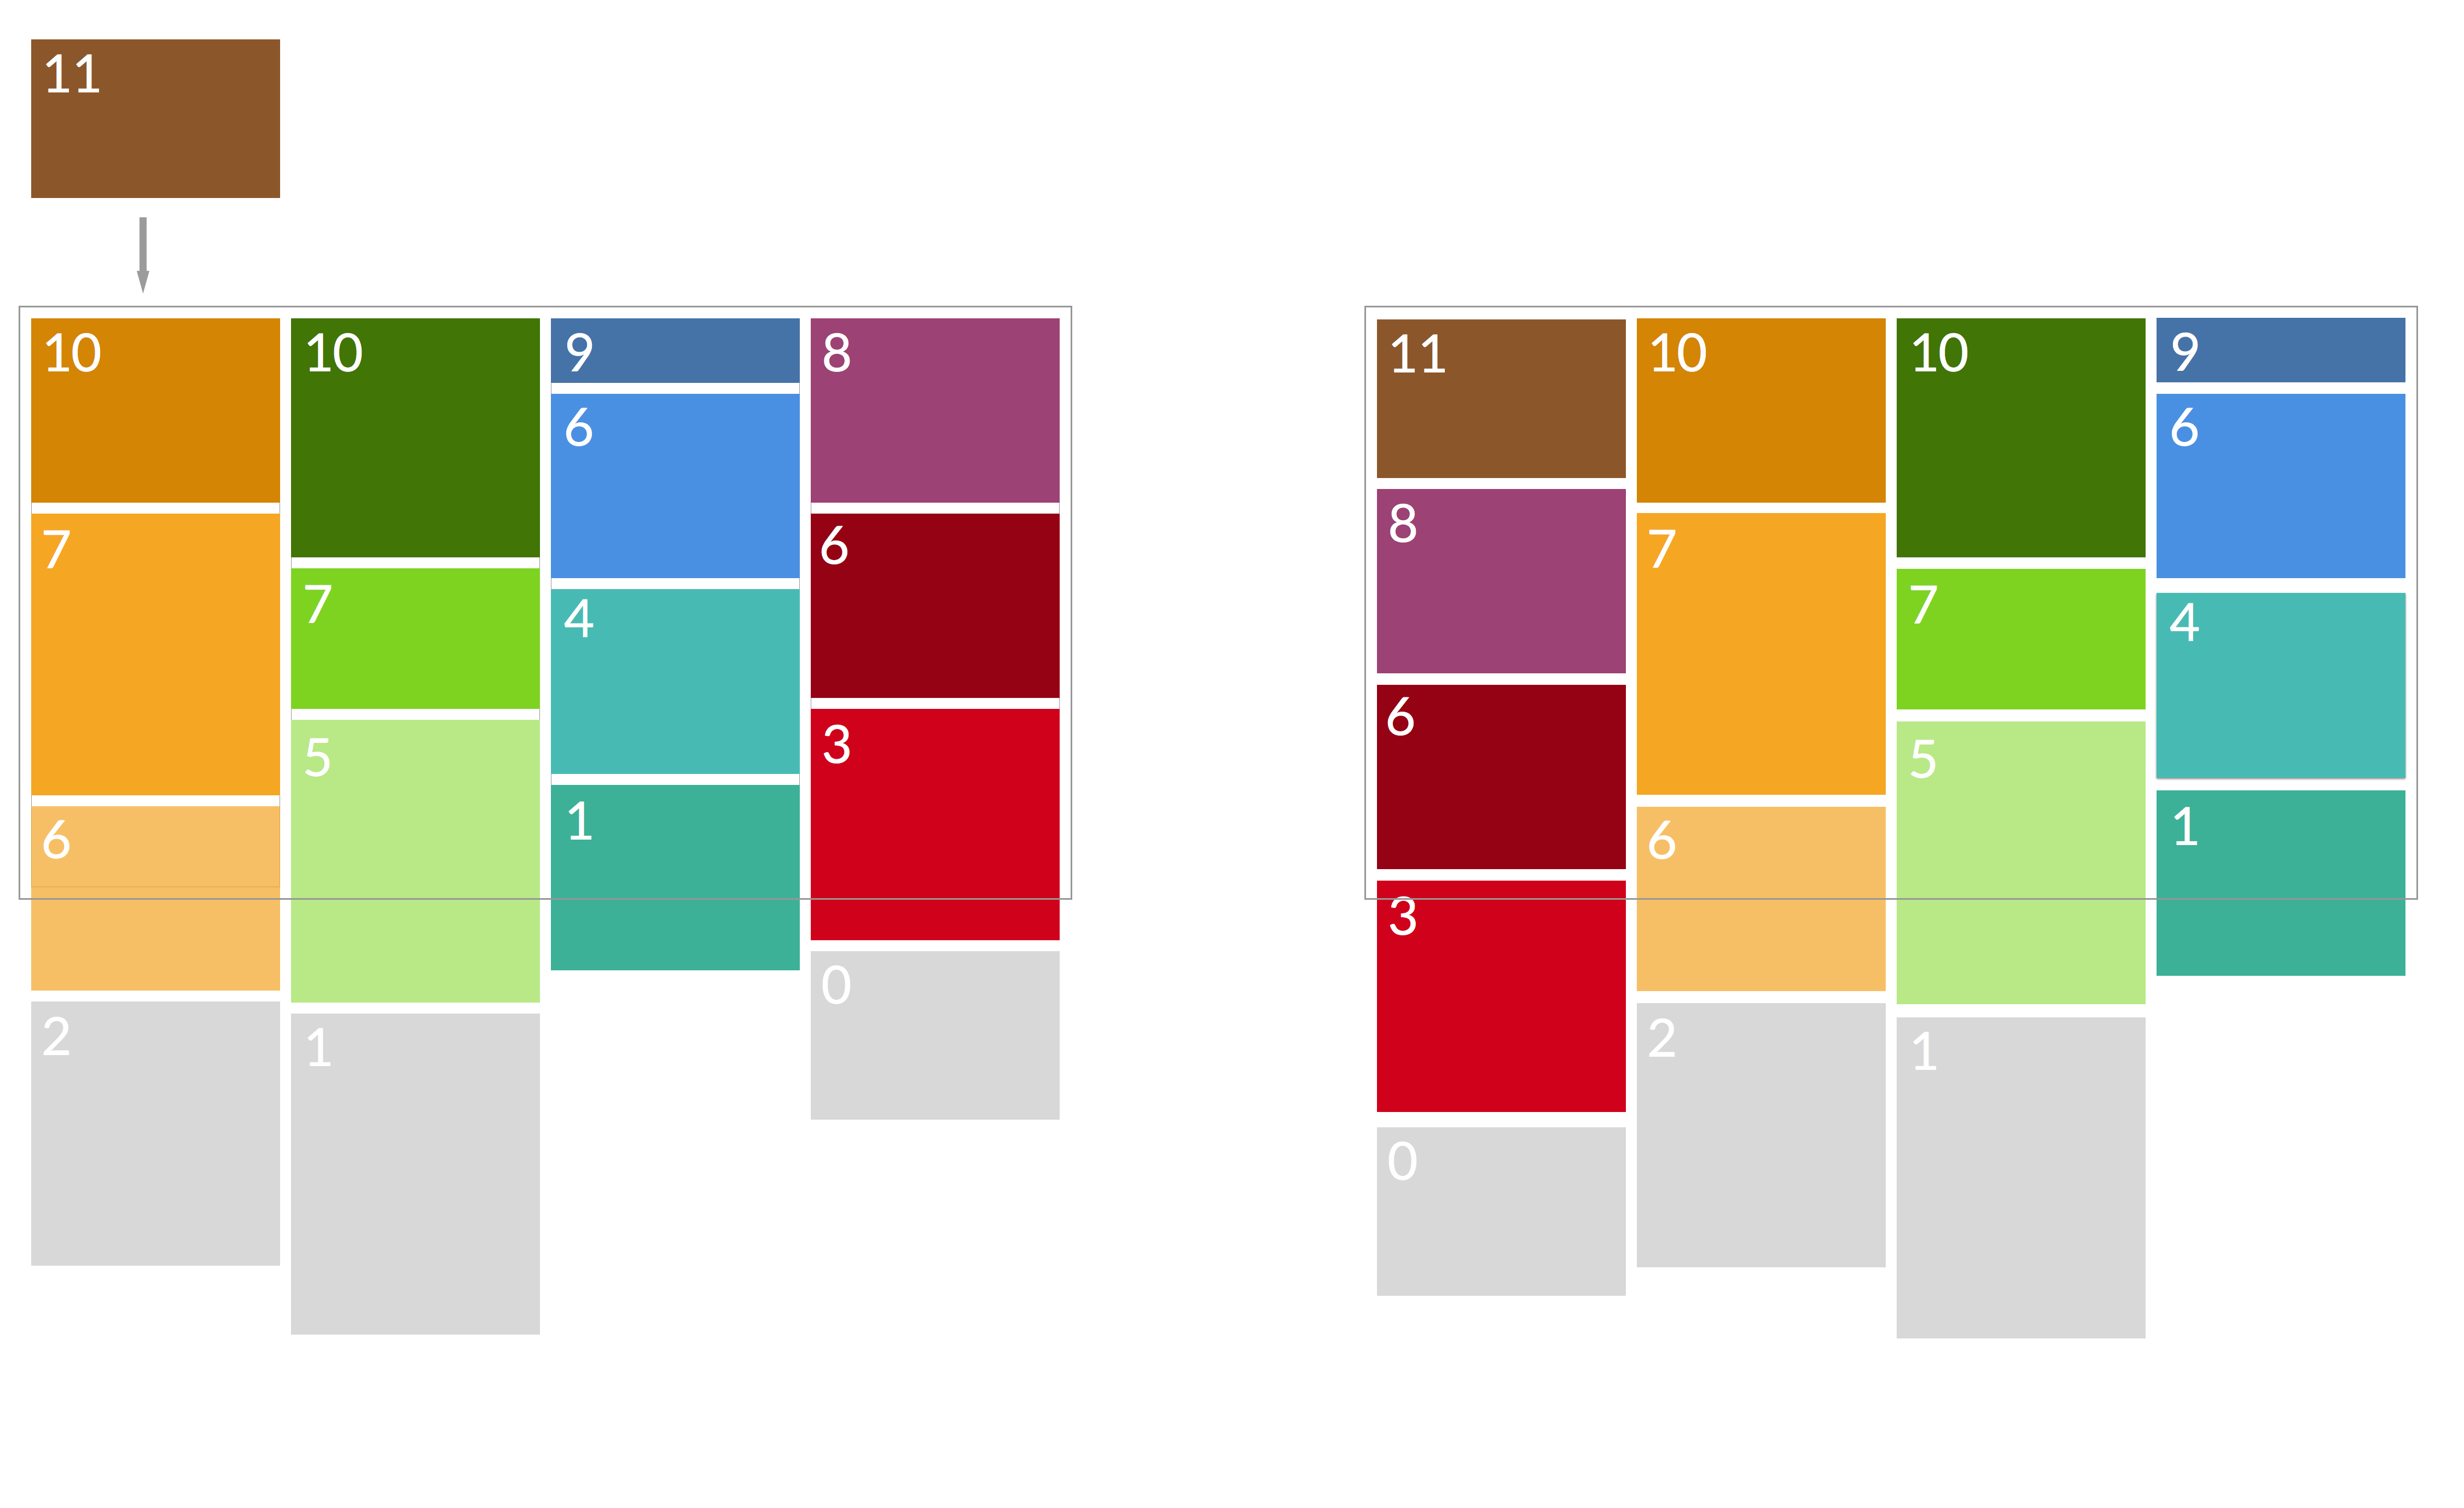
\includegraphics[width=0.8\textwidth]{images/livewall_sort.png}
    \caption{Links wird eine neue Kachel eingefügt die die höchsten Wert besitzt von allen Kacheln, rechts ist das Ergebnis bei Beibehaltung der Sortierung von links nach rechts.}
    \label{fig:livewall_sort}
  \end{figure}
  
Man kann den optimalen Fluss nur behalten indem man die Sortierung Spaltenweise macht, dazu müssen jedoch die Kacheln auf eine Spalte festgesetzt werden z.B. mittels einer Hash-Funktion oder einem simplen Modulo. Dies kann zu verwirrenden Ergebnissen führen, auch wenn es ästhetisch die beste Variante ist.

  \item \textbf{Rasterbasierte Anordnung}
  Bei dieser Form werden die einzelnen Datenpunkte in einem einheitlichen Raster dargestellet, d.h. die darstellende Fläche wird in einem Raster der Größe $(a, b)$ unterteilt, die Kacheln können nun die Größe $(x, y)$ mit $ x \in \{1, \dots, a, y \in 1, \dots, b$ besitzen.

  \begin{figure}[H]
    \centering
    \includegraphics[width=0.8\textwidth]{images/livewall_grid.pdf}
    \caption{links: Das Raster des Grids, rechts: eine zufällige Benutzung des Grids}
    \label{fig:awesome_image}
  \end{figure}

  \textbf{Vorteile} \\
  \begin{itemize}
    \item Ansprechendes Aussehen
    \item Wichtigkeit kann durch die Größe der Kachel dargestellt werden
    \item Unterschiede in der Darstellung gleicher Datenpunkte durch unterschiedliche Größe
    \item Vorteilhaft bei der Anzeige ohne Interaktion, da es keine abgeschnittenen Inhalte gibt wie bei dem Spaltendesign
  \end{itemize}

  \textbf{Nachteile}\\
  \begin{itemize}
    \item komplexes Fluss-Verhalten bei neuem Inhalt.
    \item Es müssen komplexere Methoden benutzt werden um Löcher zu verhindern
    \item Es müssen Darstellungen für die verschiedenen Kachelgrößen erstellt werden
    \item unterschiedliche Darstellungsformen können unübersichtlich wirken
  \end{itemize}

  \subsection{Probleme beim Flow-Verhalten}
  Das Flow-Verhalten beim einfügen neuer Inhalte ist bei einem grid-basierten Layout mit unterschiedlichen Kachelgrößen äußerst komplex, im ersten Schritt müsste das Behälterproblem gelöst werden und im zweiten Schritt müssten die Elemente anhand ihrer Bewertung nochmals sortiert werden. Die Lösungen des Behälterproblem darauf hin zu optimieren das der optische Fluss der Elemente minimiert wird ist keine triviale Aufgabe, weshalb man sich mit den \textit{schlechten} Lösungen zufrieden geben muss. Die JavaScript-Bibliothek packery\cite{packery} implementiert den ersten Schritt und ordnet die Elemente anhand einer Lösung des Behälterproblems, bei deren \texttt{prepend}-Methode kann sehr gut erahnt werden wie \textit{verwirrend} der Fluss bei jedem neuen Element wäre, siehe \ref{fig:grid_flow}.

  \begin{figure}[H]
    \centering
    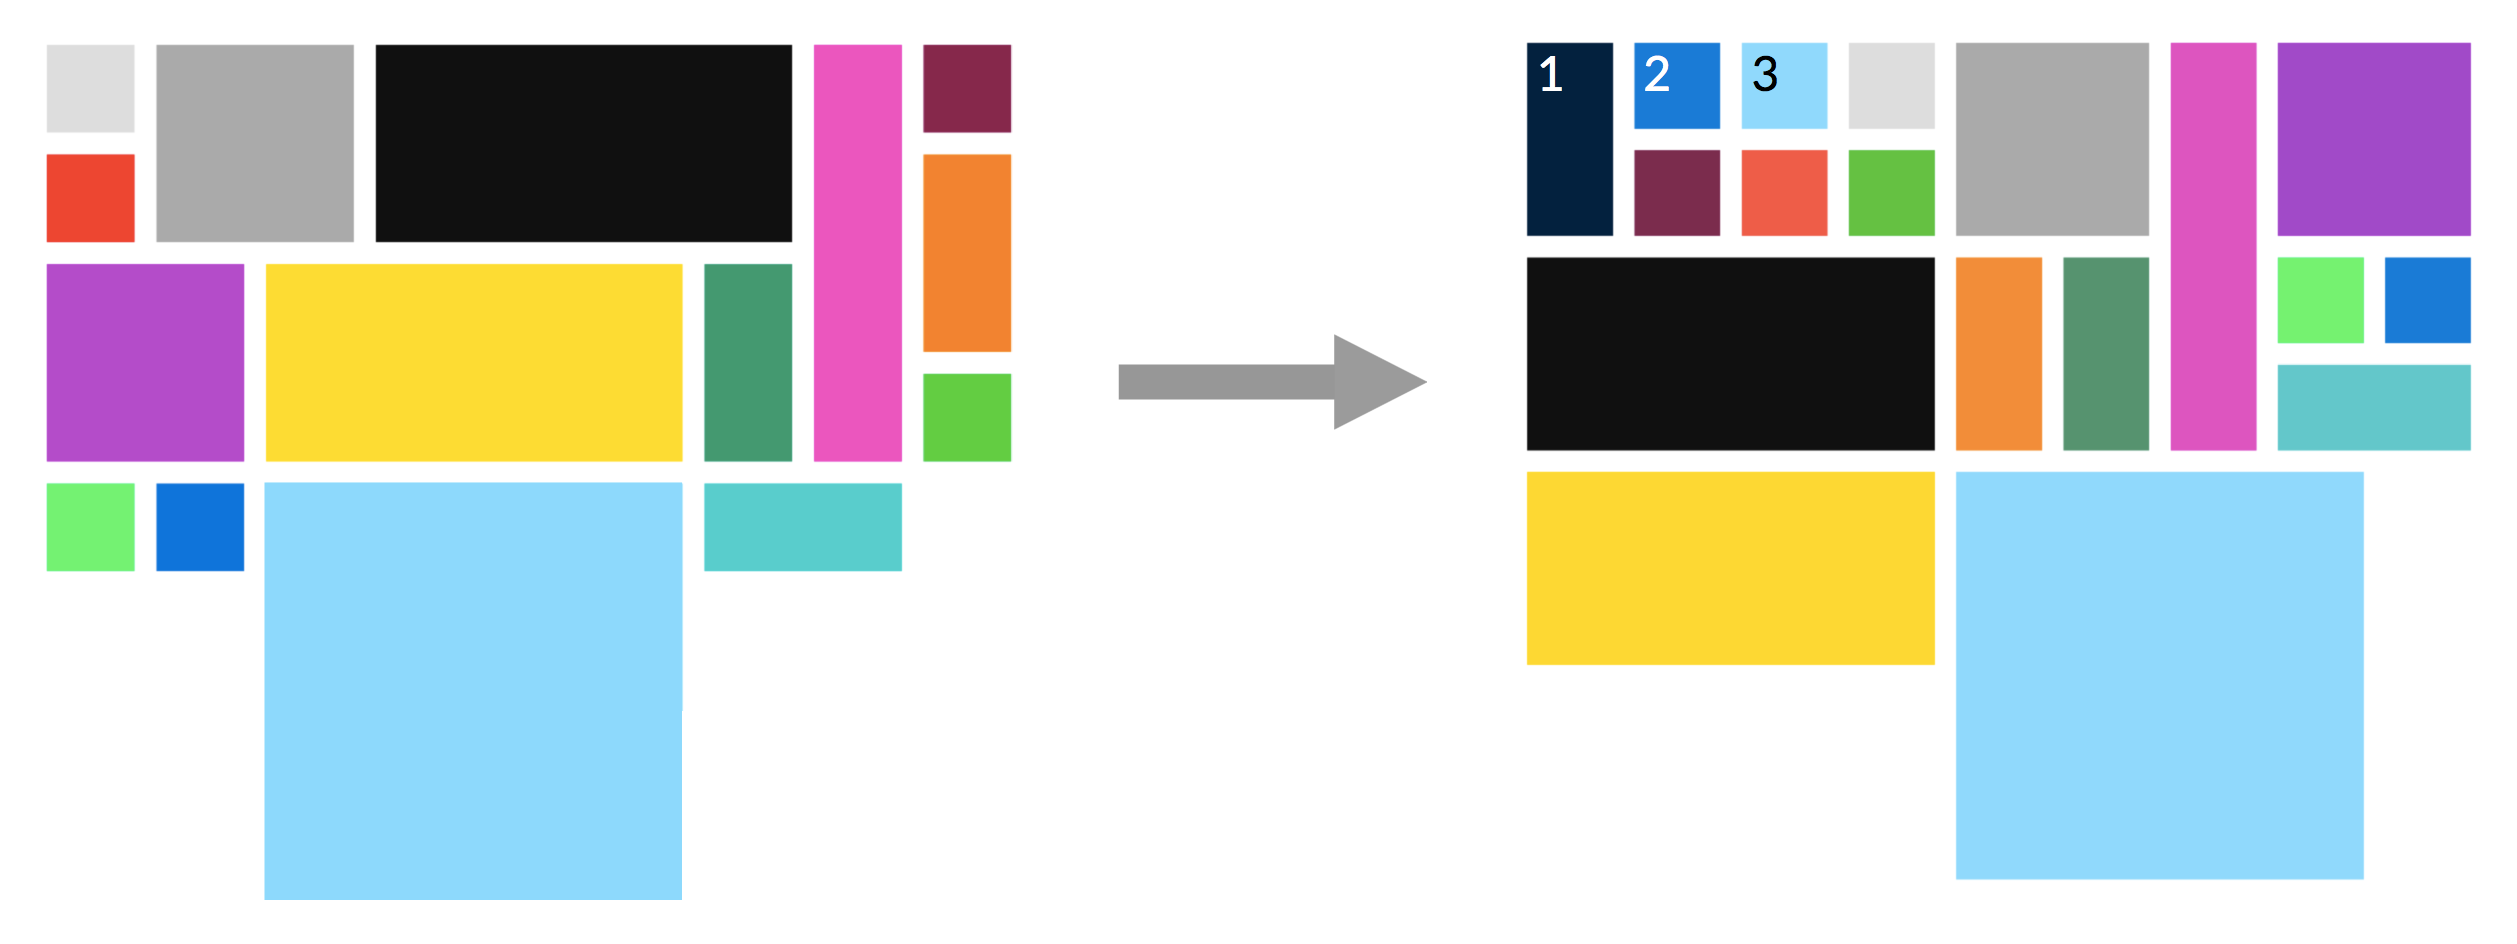
\includegraphics[width=0.8\textwidth]{images/grid_flow.png}
    \caption{Zu dem Grid links wurden die Elemente 1, 2 und 3 hinzugefügt. Das resultierende neue Layout ist rechts zu sehen. Dies ist ein praktisches Beispiel welches mithilfe von packery gemacht wurde.}
    \label{fig:grid_flow}
  \end{figure}


\end{itemize}

\subsection{Animationen}

Sinnvolle Animationen sind in den letzten Jahren immer mehr benutzt worden um die Nutzererfahrung zu verbessern, Vergleich hier zu Googles Material Design bei dem dies ein integraler Bestandteil des neuen Design-Konzeptes ist.
So war es auch hier eines der gesetzten Ziele Animationen zu entwickeln die neben dem rein ästhetischen Aspekt einen Vorteil im Verständnis des Datenflusses der Applikation ermöglichen.

\begin{enumerate}
  \item Neue Kacheln sollen von \textit{oben} kommen um einerseits zu zeigen dass es neue Inhalte gibt und andererseits um das vertraute Konzept zu benutzen dass neue Dinge von oben kommen sollten, Beispiele im echten Leben sind z.B. Börsenticker, Nachrichtenseiten oder die Abfahrttafeln am Bahnhöfen.
  
  \item Die neuen Kacheln ordnen sich an ihrem Platz ein, alte Kacheln machen dementsprechend Platz.
  \item Die Anzahl an Bewegungen soll minimal sein um nicht unnötig vom eigentlichen Inhalt abzulenken.
\end{enumerate}

Nur das Spaltenbasierte Layout erfüllt diese Anforderungen für Animationen, da die Neuberechnung des Layouts bei dem Kachelbasierten zu aufwändig ist, als dass nachverfolgt werden kann wie die Kacheln sich bewegen und welchen Gesetzmäßigkeiten sie unterliegen.

\subsection{Kacheln}\label{sec:tiles}

Das Design der Kacheln ist neben derer Anordnung die wichtigste Design-Entscheidung. Neben dem rein funktionalen Aspekt ist auch das Aussehen wichtig um z.B. die einzelnen Inhalte gut voneinander zu unterscheiden und den Benutzer nicht zu überfordern.

Rein funktional besitzt eine Kachel folgende Anforderung:

\begin{itemize}
  \item Anzeige des gefundenen Inhalts und Möglichkeit diesen zu öffnen. Die Anzeige des Inhalts kann variieren.
  \item Benutzer können den Inhalt favorisieren (speichern) und bewerten.
  \item Es werden Metainformationen wie der Typ des Inhalts (PDF, Kontakt, ...) angezeigt.
  \item Kacheln können schnell zu dem Suchbegriff zugeordnet werden von dem Sie stammen.
  \item Anzeige der letzten Interaktion mit der Komponente um den sozialen Aspekt der Anwendung zu verdeutlichen.
\end{itemize}

Obwohl die Kacheln je nach dargestellten Inhalt stark variieren können ist es ratsam ein einheitliches Benutzerinterface für die Benutzerinteraktionen zu bieten. Auch sollten die Metainformationen gleich angezeigt werden.
Mit diesen Anforderungen kann eine funktionale Kachel konzipiert werden, siehe \ref{fig:tile_prototype}.

\begin{figure}[H]
    \centering
    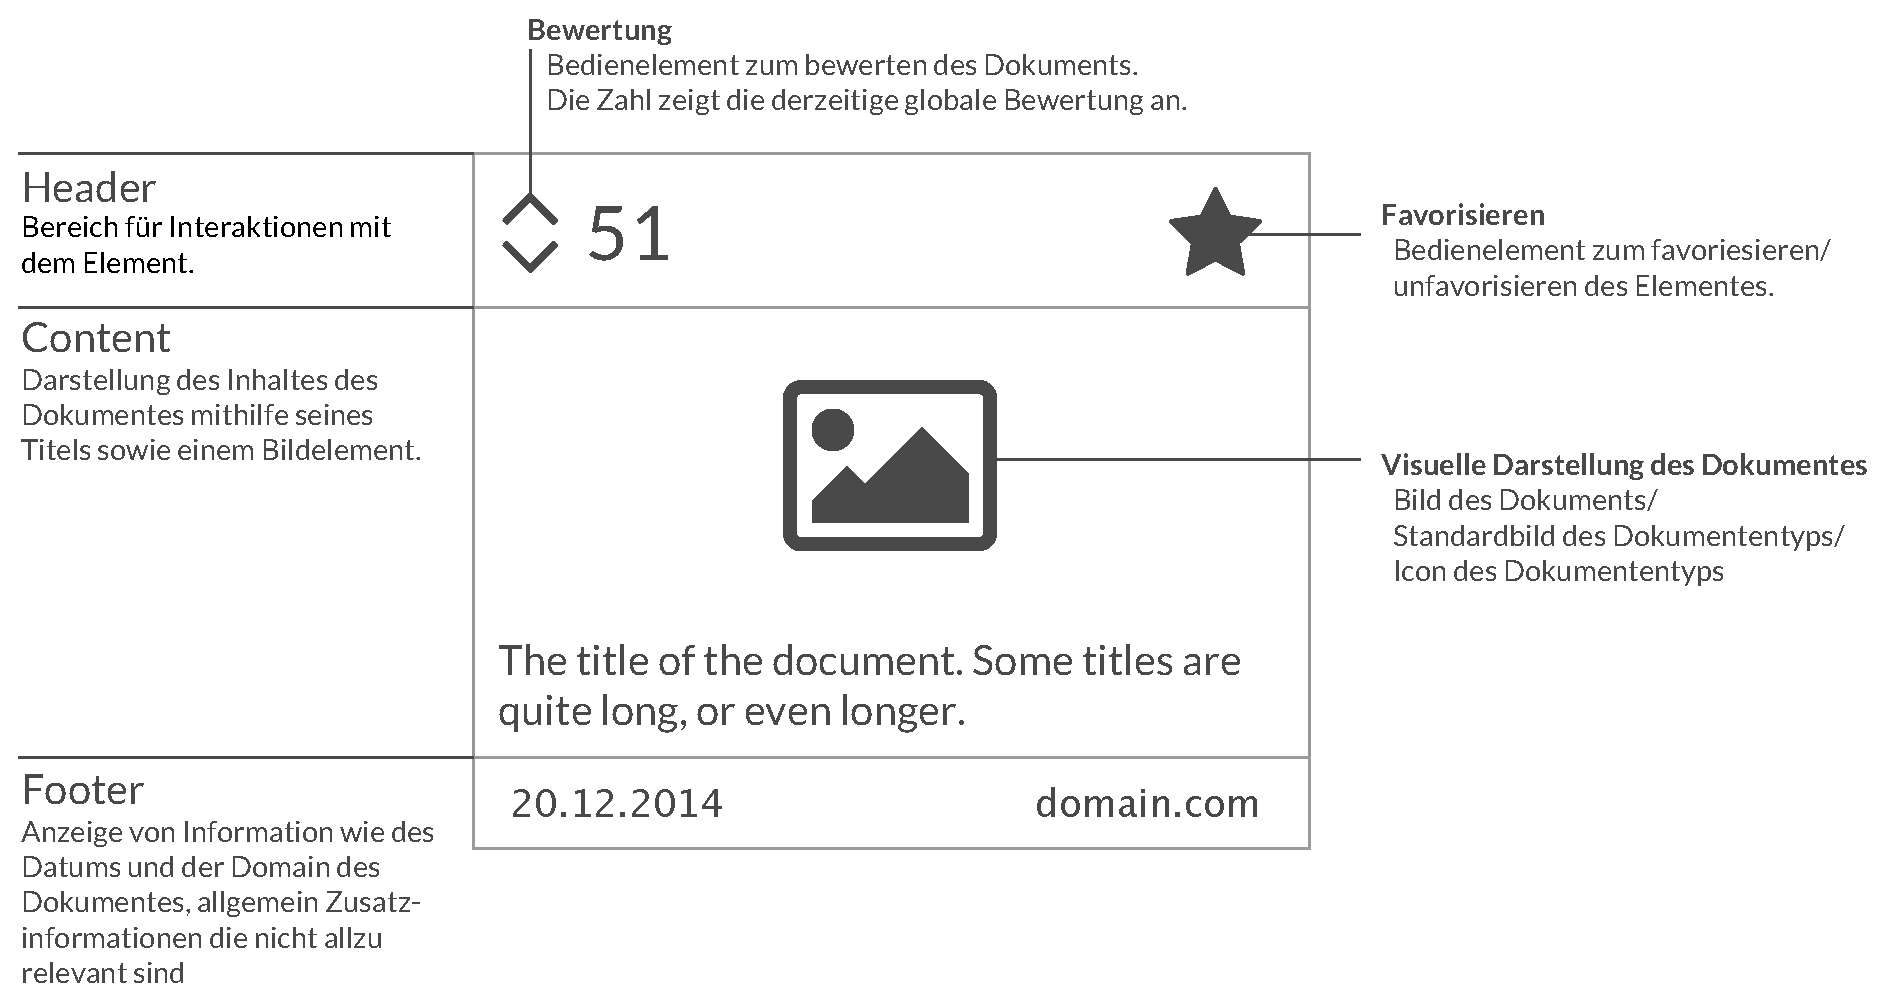
\includegraphics[width=1.0\textwidth]{images/tiles.eps}
    \caption{Eine prototyp-Kachel mit rein funktionalen Aspekten.}
    \label{fig:tile_prototype}
\end{figure}

Menschen sind äußerst gut darin Farben und unterschiedliche Formen schnell zu gruppieren, da nach aktuellem Kenntnisstand, dies Teile der ersten Verarbeitungsstufe von visuellen Informationen ist \citep{treisman1987merkmale}. Da eine schnelle Assoziation von Suchbegriff und Kachel äußerst wichtig ist, wurde die Hintergrundfarbe der Kachel dafür benutzt. Dies schränkt das Design aber insofern ein dass bis auf Grautöne und Abstufungen der verwendeten Hintergrundfarbe keine anderen Farben möglich sind, man könnte z.B. das Symbol zum Favorisieren nicht überall rot anzeigen. Doch waren das dadurch erzielte Design so überzeugend, dass dies in Kauf genommen wurde.

\begin{figure}[H]
    \centering
    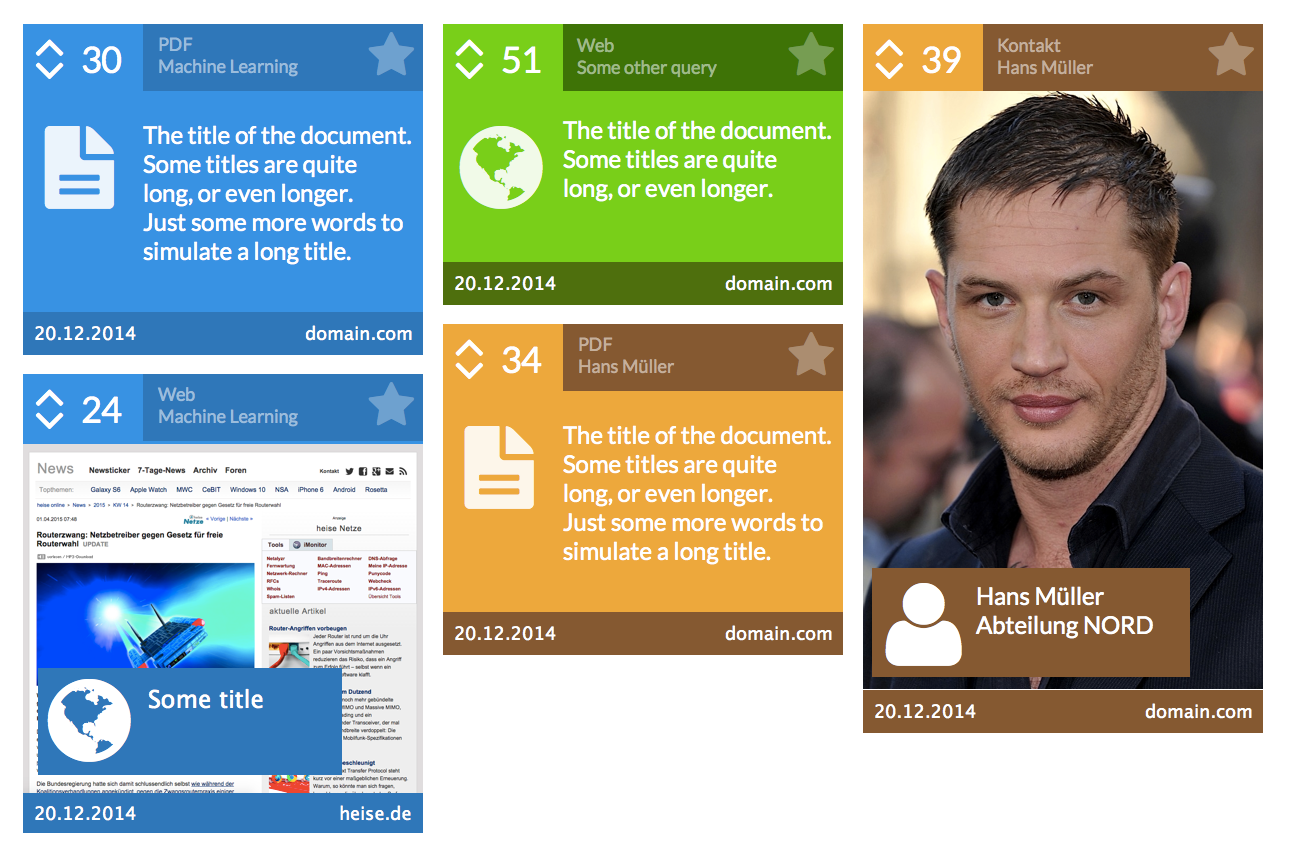
\includegraphics[width=1.0\textwidth]{images/tiles_real.eps}
    \caption{Ein erstes Design dass verschiedene Darstellungsformen für unterschiedliche Typen von Informationen benutzt.}
    \label{fig:awesome_image}
\end{figure}

\subsection{Eindeutige Zuordnung von Farben zu Suchbegriffen}

Da in \ref{sec:tiles} entschieden wurde die Hintergrundfarbe der Kacheln als Hauptunterscheidungsmerkmal der Suchbegriffe zu verwenden, muss entschieden werden wie eine Farbe zu einem Suchbegriff ausgewählt werden soll.
Alle angezeigten Farben sollten optisch zueinander gehören und miteinander harmonieren, um dies zu erreichen gibt es verschiedene Ansätze, bei allen ist jedoch der \textit{erste} Schritt die Konvertierung der Suchbegriffe zu einer Zahl. Diese Funktion sollte die typischen Eigenschaften einer \text{guten} Hash-Funktion mitbringen: gleichmässige Verteilung der Funktionswerte auf den Zielraum und Linkstotalität.
Die hier verwendete Funktion stammt von Dan Berstein und ist bekannt unter der Bezeichnung \textit{djb2}.

Der erste Ansatz wäre es eine Liste mit zueinander harmonierenden Farben zu verwenden und jeweils eine auszusuchen. Dieser Ansatz kann jedoch nur mit einer langen Liste von Farben funktionieren, auch passiert es bei dieser Methode öfter das Suchbegriffe dieselbe Farbe zugewiesen bekommen, was äußerst unerwünscht ist. Man könnte sich nun überlegen ob komplexe Konfliktresolution betrieben werden sollte - dass wenn Suchbegriffe aufeinander kollidieren eine davon eine andere Farbe bekommt.
Dadurch wird aber verhindert das jeder Suchbegriff Konsistent die gleiche Farbe bekommt.

Der zweite Ansatz besteht darin die Farben prozedural zu erstellen,
der naivste Ansatz wäre es hierbei den Wertebereich der Hash-Funktion auf $0 - 2^{16})$ einzuschränken, das Ergebnis in Hexadezimal umzurechnen und als RGB-Farbe zu benutzen. Die dadurch entstehenden Farben sind jedoch unberechenbar und würden nur per Zufall harmonieren, es gibt auch das Problem das zu viele dunkle und helle Farben erstellt werden.
Der RGB-Farbraum ist jedoch nicht dazu geeignet die Helligkeit der entstehenden Farben zu kontrollieren, dafür sind Wahrnehmungsorientierte Modelle  die Farben durch Helligkeit, Sättigung und Farbton beschreiben deutlich geeigneter wie z.B. HSV oder HSL.
Probleme von den HSx Farbräumen sind die für den Menschen ungünstige Verteilung der Farben, da wir z.B. besser im Unterscheiden von Blautönen besser sind als welche mit Grün/Rot-Anteilen, auch variiert die Helligkeit der Farben bei Änderung des Farbtons zu sehr.
Abhilfe schaffen hier die dafür erstellen Farbräume LAB bzw. die Weiterentwicklung HCL. Diese sind jedoch nicht einfach zu benutzen, da der valide Wertebereich der Eingabeparameter je nach Kombination der Werte unterschiedlich ist. Dies macht es schwer mit diesen Farbräumen Farben zu erstellen. Es gibt im speziellen um den Chroma-Wert, dieser kann grob mit der Helligkeit verglichen werden. Der Wertebereich der Sättigung und des Farbtons sind vom Chroma-Wert abhängig.

Die Wahl des idealen Farbraums ist damit nicht wirklich möglich, mittels HSL ist es einfach eine gute Farbskala prozedural zu erstellen, der Farbbereich ist jedoch ungünstig für den Menschen. LAB/HCL bieten die beste Farbverteilung für die menschliche Wahrnehmung, sind jedoch äußerst schwer zu benutzen. Eine mögliche Kombination der Vorteile beider Farbräume zeigt \citep{husl}, hier wird ein Farbraum mit der Bezeichnung \textit{human-friendly HSL} vorgestellt.

Doch keiner der Farbräume konnte eine \textit{ideale} Farbskala erstellen, es konnten in allen Farbräumen sehr anspruchsvolle Farbskalen mit wenig Kollisionen erstellt werden. Da Farbskalen ein subjektives Thema sind wurde die Möglichkeit eingebaut diese in der Applikation zu verändern - dies wurde gleich mit dem Gamification-Aspekt verbunden wodurch man nach und nach neue Freischalten kann und sich die aussuchen kann die einem am besten gefallen.

Zum testen der Farbskalen wurde eine Liste an möglichen Suchbegriffen benutzt, die Ergebnisse sind in \ref{fig:colors} zu sehen.

\begin{figure}[H]
    \centering
    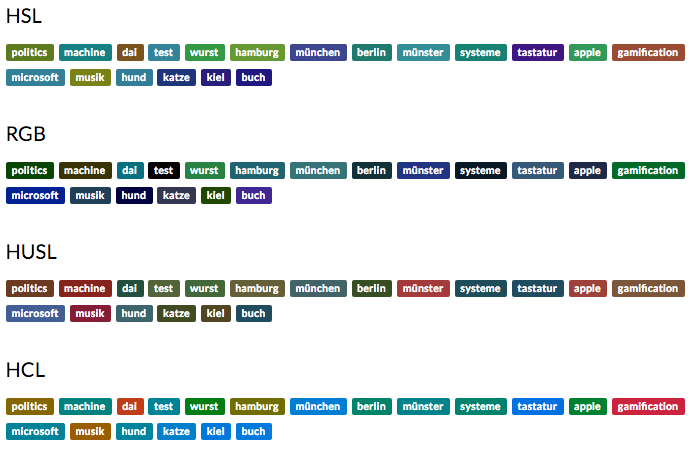
\includegraphics[width=1.0\textwidth]{images/colors}
    \caption{Farbskalen die mit verschiedenen Farbrepräsentationen erstellt wurden.}
    \label{fig:colors}
\end{figure}

\section{Gamification}

Wie in der Einleitung erwähnt ist Gamification eine mittlerweile weitverbreitete und äußerst effektive Technik um das sogenanntes \textit{User-Engagement} erhöhen, allein durch Gamification konnte z.B. die Seite DevHub ihre \textit{Engagement}-Rate um 20\% steigern \citep{zichermann2011gamification, 17}. Zahlreiche StartUps feiern große Erfolge mit dem hinzufügen von Gamification zu anstrengenden bzw. langweiligen Aufgaben, wie z.B. das Lernen einer Sprache (Duolingo\footnote{https://de.duolingo.com/}) oder Programmieren Lernen (Codecademy\footnote{http://www.codecademy.com/}).

Doch was ist Gamification eigentlich? Der Begriff entstand erst 2008 und hat seitdem viele Bedeutungen erlangt, \citep{deterding2011game} bemühten sich eine einheitliche Definition zu finden, die auch im folgenden Kontext verwendet wird.

\begin{quote}
	``Gamification'' is the use of game design elements in non-game contexts.
\end{quote}

Das Infoboard dient als Interface für Unternehmensinterne Suchmaschinen, welches zu besserem Wissensaustausch führen soll. Dies ist offensichtlich ein nicht-Spiele-Kontext der durch erhöhtes \textit{Engagement} positive Effekte für ein Unternehmen erzielen kann.
Mit dem Einsatz von Gamification-Elementen werden von uns zwei Ziele verfolgt, einerseits soll durch die Verspielisierung der Applikationsmechaniken deren Benutzung erhöht werden bzw. soll ein konstanteres \textit{User-Engangement} erzielt werden, andererseits sollen die Mechaniken zur Bewertung der Suchergebnisse gefördert werden wodurch diese noch besser werden.

% Es ist schwer neue Technologien im Unternehmensfeld einzuführen, vor allem wenn sie freiwillig benutzt werden können - so wie das hier entwickelte Enterprise Infoboard. Ziel ist es also durch die Gamification der Benutzung die Benutzer dazu zu motivieren die Anwendung gewohnheitsmäßig zu benutzen.

Die Grundlage jedes Spieledesigns ist der \textit{Compulsion Loop} welcher eine modellierte Kette an Aktivitäten darstellt, die gewohnheitsmäßig wiederholt werden um eine neurochemische Belohnung zu erhalten.

Nach \citep{gamasutra} besteht diese modellierte Kette aus 3 Schritten:

\begin{enumerate}
  \item \textbf{Anerkennung der Leistung} Die Ausführung der Aktionen wird belohnt, der Benutzer bekommt etwas was er gerne möchte. Die Herausforderung hierbei ist es etwas zu erschaffen, dass der Benutzer möchte und die Belohnung so einzuteilen das er gerade soviel bekommt dass es eine Belohnung darstellt. Am Beispiel des Rollenspieles wäre eine Belohnung z.B. die verbesserte Rüstung mit der der gespielte Charakter widerstandsfähiger wird und neue bisher verschlossene Abenteuer bestreiten kann.
  \item \textbf{Belohnung einer Aktion} Jede Aktion die der Benutzer ausführt hat eine direkte Belohnung zur Folge, diese ist jedoch so klein, dass sie direkt keine Glücksgefühle auslöst sondern erst eine Anhäufung der Belohnungen führt dazu dass der Benutzer die eigentliche \textbf{Belohnung der Leistung} erhält. Es ist zu beachten dass diese direkten Belohnungen nicht allzu schnell die Möglichkeit freischalten sie gegen dass einzutauschen wonach der Benutzer strebt. Dies könnte im Rollenspiel das Gold sein, dass benötigt wird um eine neue Rüstung zu kaufen.
  \item \textbf{Aktion} Die Aktion ist die Grundlage der Schleife, Aktionen sind das was der Benutzer ausführen soll. Im Rollenspiel könnte dies z.B. das lösen von Aufträgen sein.
\end{enumerate}

Im folgenden wird für die Gamification des Infoboard anhand dieser Schritten modelliert.

\subsection{Aktionen und deren Belohnung}

Das Infoboard besitzt ausgewählte Interaktionsmöglichkeiten die alle Teil der Aktionen sind die eine Belohnung geben.

\begin{itemize}
  \item Bewertung der Suchergebnisse
  \item Favorisieren von Suchergebnissen
  \item Eingabe und Löschung von Suchbegriffen
  \item Anmeldung und Abmeldung
\end{itemize}

Durch einige dieser Aktionen wird der User Punkte bekommen, z.B. ist es häufig üblich für das tägliche Besuchen der Seite dem Benutzer Punkte gutzuschreiben. Wichtig für uns ist es, dass die Bewertung der Suchergebnisse besonders gefördert wird, womit es denkbar ist hier eine größere Punktzahl im Vergleich zu den anderen Aktionen vergeben wird.

\subsection{Anerkennung der Leistung}

Die Leistung des Benutzers muss anerkannt werden, im folgenden werden verschiedene Ansätze für Punkte/Bestenlisten und Abzeichen gezeigt und erklärt warum wir uns für den einen oder anderen Ansatz entschieden haben.

\subsubsection{Punkte}
Punkte sind unerlässlich im Spielekontext, auch wenn die Punkte für den Benutzer nicht mal sichtbar gemacht werden sind sie wichtig um dem Spieledesigner die Möglichkeit zu geben das System zu evaluieren und daraufhin zu verändern \cite{zichermann2011gamification, 36}. Nach \citep{zichermann2011gamification, 38} unterscheidet man erhaltene Punkte in folgende Kategorien.

\begin{itemize}
	\item Erfahrungspunkte
    \item Eintauschbare Punkte
    \item Fähigkeitspunkte
    \item Karmapunkte
    \item Ansehenspunkte
\end{itemize}


Anstelle eines komplexen Spielesystems wo verschiedene Punktesysteme benutzt werden, wurde hier entschieden nur eine Art von Punkten zu benutzen, welche größtenteils auf den Erfahrungspunkten aufbaut. Erfahrungspunkte stellen die wichtigste Kategorie von Punkten dar, jede Interaktion des Benutzers wird mittels Erfahrungspunkte festgehalten (\citep{zichermann2011gamification, 38 - 39}) und geben bei einer bedachten Punktevergabe  eine gute Quantifizierung der Leistung des Benutzers womit man Erfahrungspunkte gleichzeitig für eine Bestenliste benutzen kann - und damit als eine Art Ansehenspunkte. Um den Punktemechanismus noch etwas spannender zu gestalten, kann man sie für sogenannte \textit{Booster} eintauschen durch welche jeder Erhalt von Punkten für einen gewissen Zeitraum mit einem Multiplikator erhöht wird z.B. erhält der Benutzer für einen Tag die doppelte Anzahl an Punkten.

Die Idee hinter den Boostern ist es den Compulsion-Loop daraufhin zu unterstützen dass der Nutzer sie kaufen wird um seine Punktzahl noch weiter zu erhöhen. Durch die kurze Verweildauer des Boosters und dem Ziel des Benutzers seine Punkte zu erhöhehn, wird dieser zwangsläufig seine Nutzung mit dem System erhöhen, da sich der Booster sonst nicht gelohnt hätte.

Die Punkte sind für den Benutzer immer sichtbar und aktualisieren sich in Echtzeit sobald der Benutzer eine Aktion ausführt die Punkte bringt. Zudem werden sie auf der Abzeichenseite nochmals angezeigt, wobei ein Balkendiagramm eine genauer Kategorisierung anzeigt, woher der Benutzer diese Punkte überhaupt hat, siehe \ref{fig:points}.

\begin{figure}[H]
    \centering
    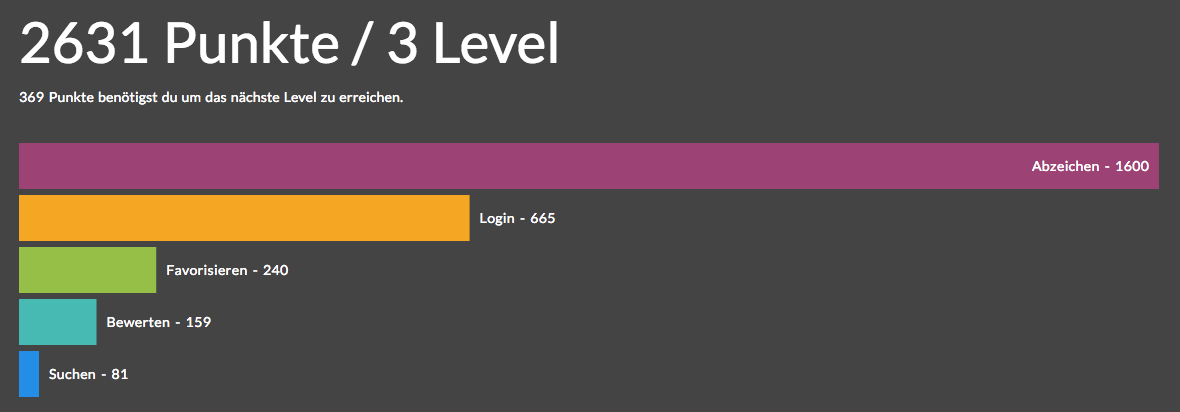
\includegraphics[width=0.8\textwidth]{images/infoboard_userstats.png}
    \caption{Die Punkte des Benutzers aufgeteilt in Kategorien.}
    \label{fig:points}
\end{figure}

Zusammengefasst benutzen wir \textbf{Erfahrungspunkte} die für alle Aktionen vergeben werden und für \textit{Booster} ausgegeben werden können. Bestenlisten ermöglichen einen Vergleich der Punkte zu anderen Benutzern.

\subsubsection{Bestenliste}

Der Sinn von Bestenlisten ist es einen einfachen Vergleich von Dingen (in unserem Fall Benutzern) zu bieten. Bestenlisten sind zu so einem integralen Bestandteil unseren alltäglichen Lebens geworden, dass wir sofort eine erkennen wenn wir eine sehen. Beispiele für Bestenlisten im echten Leben umfassen die Ergebnisse der Stiftung Warentest, Klausurnotenhaushänge oder die Bundesligatabellen.

Nach \citep{zichermann2011gamification, 50 - 51} kann man zwischen zwei Arten von Bestenlisten unterscheiden, die \textit{lass-dich-nicht-entmutigen} und die \textit{unendliche} Bestenliste. Bei ersterer wird der Benutzer, egal welchen Platz er in der Bestenliste inne hat, immer direkt in die Mitte angezeigt. Hierbei ist es irrelevant ob er Platz 43 oder 40000 ist, er sieht sich selbst immer in der Mitte der Liste, um sich herum sieht er seine direkte Konkurrenz. Wenn der Benutzer auf einen der Top 10/20/30 Plätze kommt sollte sich dieses Verhalten jedoch ändern und er sollte die \textit{korrekte} Liste sehen.
Bei der \textit{unendlichen} Bestenliste werden alle Benutzer angezeigt, es gibt jedoch meistens die Möglichkeit die Anzahl der Benutzer zu verringern, so hat z.B. das Spiel Doodle Jump 3 Arten des Leaderboards: Lokal, Freunde und Global.

Ein weiterer Aspekt ist der Zeitraum der angezeigt wird. Vor allem bei Applikationen bei denen die Punktzahl immer weiter akkumuliert werden kann und demnach unendlich Punkte zulassen, kann eine Bestenliste die auf dem kompletten verfügbaren Zeitraum aufbaut für Neuanfänger entmutigend wirken da sie es wohl nie schaffen werden einen höheren Platz zu erreichen wenn jeder doch gleich viele Punkte pro Tag erzielen kann.
Eine offensichtliche Lösung wäre es den Zeitraum auf z.B. die letzte Woche zu beschränken, was dann aber einen ähnlich negativen Effekt auf die dauerhaften Nutzer haben würde: Sie könnten ihre Vormachtstellung nicht demonstrieren.

Wir haben uns deswegen entschieden immer 2 Bestenlisten anzuzeigen: Der komplette Zeitraum und die letzten 30 Tage. Dadurch ist es möglich beide Parteien zufrieden zu stellen ohne Kompromisse eingehen zu müssen. Es werden ebenfalls beide Arten der Bestenliste benutzt: Im persönlichen Dashboard wird die \textit{lass-dich-nicht-entmutigen}-Bestenliste und in den globales Statistiken wird eine \textit{unendlichen} Bestenliste benutzt, siehe \ref{fig:leaderboarduser} für die \textit{lass-dich-nicht-entmutigen}-Bestenliste.

\begin{figure}[H]
    \centering
    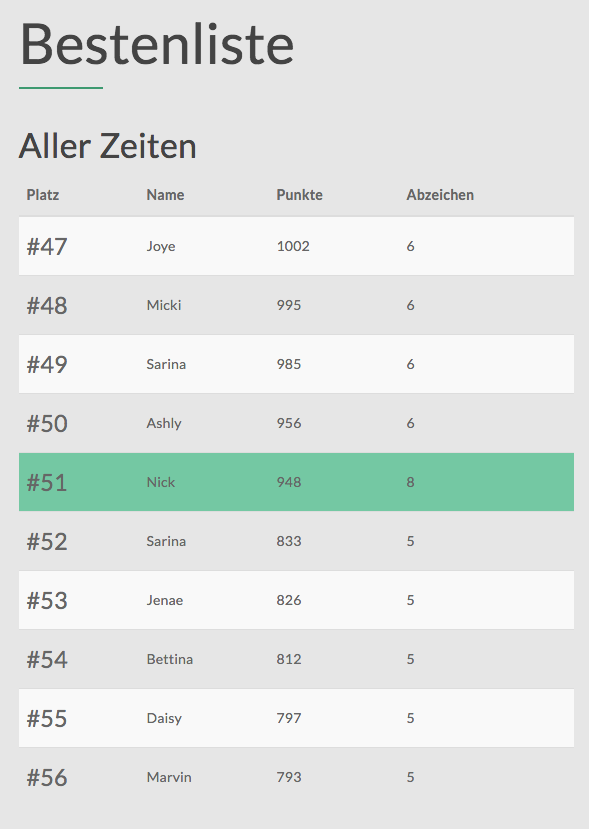
\includegraphics[width=0.5\textwidth]{images/infoboard_leaderboard_user.png}
    \caption{Die Benutzerzentrische Bestenliste, hier sieht sich der Benutzer immer in der Mitte der Liste.}
    \label{fig:leaderboarduser}
\end{figure}

\subsection{Abzeichen}

Abzeichen bzw. Badges sind ein etabliertes Element der Gamification. Nach \citep{zichermann2011gamification, 55} nutzen sie viele Eigenschaften der menschlichen Natur um begehrenswert zu sein: das menschliche Sammelverhalten, die plötzliche (positive) Überraschung wenn ein unerwartetes Abzeichen erhalten wurde, Sozialer Status (ähnlich zu Punkten), Pure Ästhetik der Abzeichen und das Aufgabenziel das hinter jedem Abzeichen steckt.

In manchen Fällen sind Abzeichen so effektiv eingesetzt dass sie sogar Level ersetzen - z.B. mit speziellen Level-Abzeichen, als Beispiel sei Foursquare gennant bei der der Benutzer das Abzeichen für das erreichen einer bestimmten Anzahl an \textit{check-ins}\footnote{Der Begriff \textit{check-in} wird von vielen sozialen Diensten benutzt um an sich an einem realen Ort ``einzuchecken'' - um dies z.B. seinen Freunden mitzuteilen} erhält. Dies funktioniert bei Foursquare darum gut, da \textit{check-ins} der wichtigste Bestandteil der Applikation sind \citep{zichermann2011gamification, 57}. Auch haben \textit{check-ins} keine negative Konnotation da es zumeist als überaus positiv angesehen wird wenn man häufig ausgeht und neue Orte kennen lernt und man damit auch gerne zeigt wie viele \textit{check-ins} man schon hatte.

Trotz aller positiven Aspekte von Abzeichen sind sie nicht einfach zu benutzen, so benutzt \citep{zichermann2011gamification, 56} den Begriff ``badgenfreude'' für ein Konzept, bei dem zu viele langweilige und sinnlose Abzeichen den Sinn von Abzeichen zunichte machen und negative Folgen für das \textit{User Engagement} haben können.

Es ist sehr wichtig dass die Abzeichen den Benutzer nicht stören, er soll es mögen sie zu bekommen. Aber wann mag es ein Benutzer Abzeichen zu bekommen und wann fangen sie an zu stören?
Als erstes kann man die Frequenz des Erhalts betrachten, um anfangs den Benutzer zu motivieren gibt man ihm am Anfang meistens relativ viele Abzeichen, so ist es typisch ein Abzeichen für die erste Anmeldung oder die erste geschaffene Herausforderung zu geben.
Die Frequenz muss jedoch mit der Zeit nachlassen, damit sie den Benutzer nicht von der eigentlichen Applikation ablenken und damit die Abzeichen weiterhin als wertvoll betrachtet werden.
Es sollte für den Benutzer weiterhin immer offensichtlich sein wofür er ein Abzeichen bekommen hat und welchen Wert es besitzt. Der Wert des Abzeichens sollte graphisch repräsentiert werden z.B. werden sehr oft die Farben Bronze/Silber/Gold als Analogie zu Medaillen benutzt um den Wert zu symbolisieren.
Damit der Benutzer weiß welche Abzeichen es noch gibt und wie er sie erhalten kann, sollte es möglich sein alle erhältlichen Abzeichen mit einer jeweiligen Beschreibung wie man es denn erhält einzusehen.

\begin{figure}[H]
    \centering
    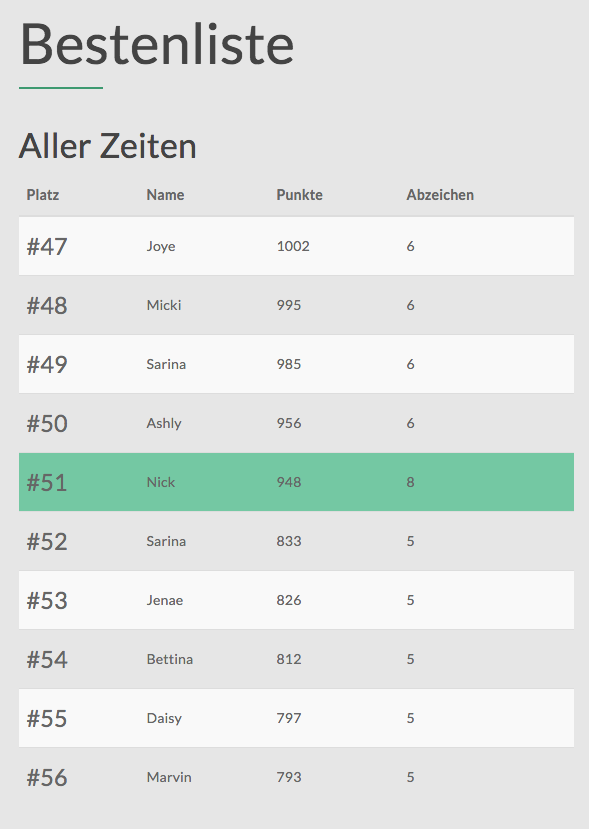
\includegraphics[width=0.6\textwidth]{images/infoboard_leaderboard_user.png}
    \caption{Die Benutzeransicht für die erhaltenen Abzeichen. Der hier gezeigte Benutzer besitzt die Favoriten-Abzeichen in allen Ausführungen.}
    \label{fig:badges}
\end{figure}

So hat sich schlussendlich folgendes Schema für die Abzeichen des Infoboards ergeben. Es gibt 3 Kategorien von Abzeichen, die jeweils eine anderen Wert darstellen. Die erste Kategorie sind leicht zu erhaltene Abzeichen, die zweite Kategorie sind mittelmäßig schwer zu erhaltene Abzeichen, d.h. wenn man das Abzeichen haben möchte kann man es auch in angemessener Zeit erhalten. Die Abzeichen der letzten Kategorie benötigen ca. 50x mehr Zeit als die der ersten, dadurch sollen auch Vielbenutzer weiterhin durch das Abzeichensystem motiviert werden. Visuell wird der Wert durch eine Krone dargestellt, wobei die der letzten Kategorie am imposantesten aussieht, siehe dazu \ref{fig:badges}.
Der Erhalt von neuen Abzeichen wird so schnell wie möglich dem Benutzer mitgeteilt werden - jede vom Benutzer ausgeführte Aktion wird an das Backend gesendet, welches \textbf{immer} berechnet ob dieser dafür ein neues Abzeichen bekommt. Ist dies der Fall wird das dem Frontend mitgeteilt und der Benutzer bekommt eine Nachricht angezeigt, siehe \ref{fig:flashmessage}. Dieser Vorgang dauert weniger als eine halbe Sekunde.
Damit das Abzeichensammeln nicht langweilig und obsolet wird, sollten regelmäßig neue Abzeichen eingeführt werden, der Quelltext wurde daraufhin optimiert damit dies nicht länger als ein paar Minuten dauert.

\begin{figure}[H]
    \centering
    
\includegraphics[width=0.8\textwidth]{images/infoboard_flashmessage.png}
    \caption{Eine gezeigte Flashmessage, diese werden benutzt um den Benutzer um ein gerade erreichtes Level oder ein neu erhaltenes Abzeichen zu informieren.}
    \label{fig:infoboard_flashmessage}
\end{figure}

\chapter{Technische Umsetzung}\label{chap:tech}

In \ref{chap:concept} wurde die Applikation soweit geplant, dass die Technische Umsetzung erfolgen kann, dies geschieht in diesem Kapitel. Viel Wert wurde darauf gelegt die getroffene Technologieentscheidungen zu begründen, wie auch die getroffene Architekturentscheidung.
Die Technische Umsetzung wird sich größtenteils mit dem Frontend beschäftigen, das Backend wird nur kurz in \ref{sec:backend} behandelt.


\section{Wahl der Technologie}

Die erste Frage die sich bei der Umsetzung stellt, ist welche Technologie verwendet werden soll.

Die Wahl der zu verwendeten Technologie ist ein wichtiger Punkt der die darauffolgende Entwicklung und spätere Wartung beeinflusst. Es wird versucht auf folgende Punkte einzugehen:

\begin{itemize}
  \item Technologie ist \textit{erwachsen} \\
  Die verwendete Bibliothek oder ähnliches ist nicht allzu neu und hat sich in vielen Applikationen bewährt, sie ist soweit ausgereift das Umgehungslösungen oder Fehlerbehebung nur in den seltensten Fällen nötig sein sollten.
  \item Die Technologie hat keine große Einstiegsbarriere \\
  Es wird versucht nicht allzu viele Frameworks zu benutzen und wenn, dann welche die weitestgehend bekannt sind und/oder in dem DAI-Labor viel benutzt werden. Wenn Bibliotheken verwendet werden, wird darauf geachtet das sie einfach zu lernen sind und intuitiv in der Benutzung.
  \item Die Technologie ist zukunftssicher \\
  Es ist immer schwer abzuschätzen welche Technologie länger überleben wird, doch wird versucht anhand von Faktoren wie Popularität, Aktivität der Entwicklung und Einsatz bei großen Firmen dies so gut wie möglich zu garantieren.
\end{itemize}

\subsection{Programmiersprache}

Die wichtigste Wahl ist die Wahl der Programmiersprache, im Frontend wird diese Entscheidung größtenteils dadurch abgenommen das Browser exklusiv die Ausführung von JavaScript beherrschen, andere Sprachen sind nur über Erweiterungen (Flash, Java) verfügbar deren Relevanz in den letzten Jahrzehnten soweit abgenommen hat, dass sie keine Option mehr darstellen.

JavaScript ist jedoch nicht die beliebteste Sprache, die Tatsache das die Sprache in ca. 10 Tagen geschrieben wurde mag dies erklären \citep{severance2012javascript}, so kam es dass JavaScript in den letzten Jahren immer mehr zu einem Kompilierungsziel geworden ist, d.h. andere Programmiersprachen kompilieren zu validem JavaScript-Code. Diese Praxis ist mittlerweile so populär geworden, dass JavaScript auch als \textit{Assembly of the Web} \cite{webassembly} bezeichnet wird. Die populärsten Programmiersprachen die zu JavaScript kompilieren sind vermutlich CoffeeScript, TypeScript und Java (mittels GWT). Die Liste der Sprachen ist jedoch endlos mit über 300-Sprachen die zu JavaScript kompilieren. Eine Auflistung dieser ist auf dem Github-repository von CoffeeScript zu finden \cite{javascriptcompile}.

\citep{zakai2011emscripten} veröffentlichten mit \textit{emscripten} das mit Abstand aufwändigste Projekt in diesem Bereich. Dies ist ein LLVM-zu-JavaScript-Kompilierer mit dem es unter anderem möglich ist C++-Quelltext zu JavaScript zu kompilieren, wodurch z.B. TeX-Compiler im Browser ausgeführt werden konnten \cite{texlive}.

Die Nutzung dieser Sprachen, vor allem der populärsten hat viele Vorteile von vereinfachter Syntax (CoffeeScript) hin zu statischer Typisierung (GWT), so bleibt die Frage ob es überhaupt noch zukunftssicher bzw. praktikabel ist reines JavaScript zu benutzen.
Die Frage kann mit einem klaren Ja beantworten werden, wenn eine Prämisse an die Ausführungsumgebung gesetzt wird: Sie unterstützt JavaScript in der Version 6, bzw. ECMAScript 6 (Im nachfolgenden mit ESx abgekürzt).
Die für JavaScript zuständige Organisation ECMA investierte viel Arbeit darein, die Tatsache dass JavaScript nur in 10 Tagen geschrieben wurde etwas weniger offensichtlich zu machen. Mit ECMAScript 6 \cite{es6} zeigt diese Arbeit am deutlichsten Früchte. Funktionalitäten wie Destructuring, Generators , Modules, Template Strings oder Promises lassen ES6 zu einer modernen Sprache werden.

Die aktuellen Browser unterstützen bisher jedoch nur einen Bruchteil der ES6 Spezifikation, eine komplette Übersicht ist unter \cite{es6features} zu finden. Es wird vermutlich noch bis in 2017 andauern bis alle aktuellen Browser ES6 ausreichend unterstützen.

Doch sind die Vorteile so überwiegend im Vergleich zu ES5, dass eine Nutzung von ES6 äußerst wünschenswert ist.
Die Lösung des Problems wurde im Grunde schon erwähnt: Man kompiliert JavaScript zu JavaScript bzw. ES6 zu ES5.
So absurd dies auch klingen mag, die Tatsache das JavaScript heutzutage immer im Zusammenhang mit Build-Tools benutzt wird die z.B. den Quelltext verkleinern oder ihn unlesbarer machen, bedeutet dass der Entwickler nur minimalen Aufwand betreiben muss damit er ES6 auch in ES5 Umgebungen benutzen kann.

So wurde für diese Arbeit entschieden, dass ES6 die beste Wahl für die Programmiersprache ist. Alle Browser werden ES6 in Zukunft unterstützen, womit ES6 keinesfalls eine obsolete Sprache werden wird. Außerdem ist im Vergleich zu den richtigen Kompilier-zu-JavaScript-Sprachen, ES6 die geringste Hürde für neue Entwickler die JavaScript schon kennen: ES6 ist abwärtskompatibel und die neuen Funktionalitäten können in ein paar wenigen Stunden gelernt werden, wenn dies überhaupt nötig ist.

Neben reinem ES6 benutzen wir jedoch auch noch eine von Facebook entwickelte Erweiterung namens JSX \cite{jsx}, diese Erweitert JavaScript mit der Möglichkeit UI-Komponenten mit einer HTML-Syntax zu beschreiben. Dies wäre z.B. valides JSX:

\begin{minted}{javascript}
	var header = <h1>Überschrift</h1>;
\end{minted}

Es mag merkwürdig erscheinen HTML-markup direkt in JavaScript zu schreiben, doch wird dadurch die Benutzung von der hier verwendeten Interface-Bibliothek React.js deutlich vereinfacht.
Bisher ist JSX ein Vorschlag von Facebook an ECMA, doch ist die Benutzung von JSX mittlerweile so verbreitet, so unterstützt eslint \cite{eslint} wie auch der ES6-ES5-Kompilierer Babel JSX \cite{babel}, dass eine Integration etwas JSX-ähnlichem ziemlich wahrscheinlich ist.
Mittels ES6-templatestrings ist es möglich \textit{Domain Specific Languages} zu schreiben, so gibt es mittlerweile auch ein proof-of-concept JSX rein in ES6 zu schreiben \cite{templatestrings}.

Neben JavaScript muss auch CSS-geschrieben werden, da CSS ebenfalls viele Mängel hat gibt es auch hier Projekte wie less oder sass, die CSS z.B. mit Variablen erweitern. Es hat sich bewährt less oder sass zu benutzen, so wurde auch für diese Applikation entschieden less zu benutzen, da damit auch Bootstrap geschrieben wurde - das hier verwendete CSS-Framework.
Das Ausmaß dieser Entscheidung ist jedoch kein Vergleich zu der Programmiersprachen-Entscheidung, weswegen es nicht lohnt die Kosten/Nutzen genauer zu betrachten.

\subsection{Ladezeiten}\label{sec:loadingtimes}

Ein großer Faktor der in anderen Umgebungen lange Zeit keine Rolle mehr spielt ist die Größe des Quelltextes. Bevor bei Javascript irgendeine Bibliothek benutzt werden kann muss sie zuerst beim Benutzer heruntergeladen und ausgeführt werden, was bei langsamen Computern mit nicht perfekter Internetverbindung ein enormer Bestandteil ist. Um den Punkt nochmal zu verdeutlichen wurde ein kleiner Test gemacht. Dazu wurde eine EmberJS-Demoapplikation ausgeführt\footnote{Auf einem Macbook Air mid 2013 in minimal Konfiguration und dem Chrome Browser in Version 41, die vorhandene Internetverbindung hatte eine Übertragungsrate von $50000 \frac{\text{bit}}{s}$} die sehr wenig wirkliche Logik besitzt, sodass gut zu zeigen ist wie viel das Herunterladen und Ausführen nur der Bibliotheken ausmachen.
Die Anwendung ist auf Github zu finden \cite{embercrud}.
\begin{figure}[H]
    \centering
    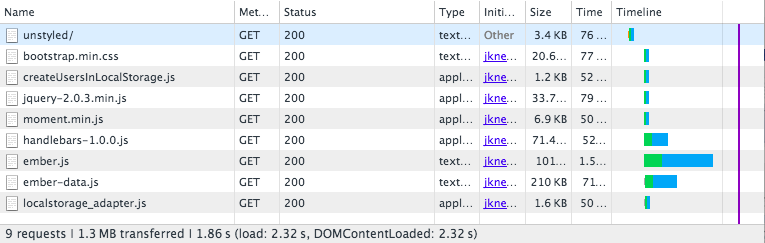
\includegraphics[width=0.8\textwidth]{images/performance_1.png}
    \caption{Übertragungszeit der benötigten Dateien}
    \label{fig:loadtimes}
\end{figure}
\begin{figure}[H]
    \centering
    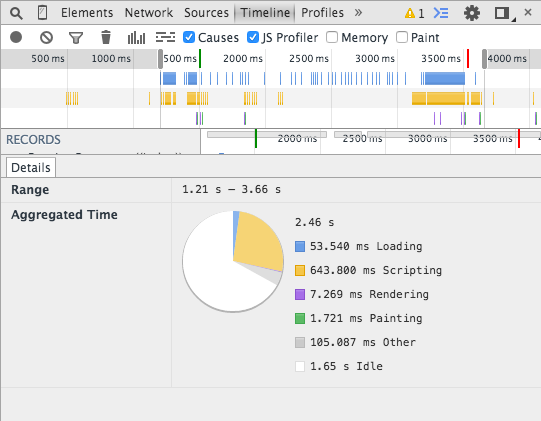
\includegraphics[width=0.6\textwidth]{images/performance_2.png}
    \caption{Benötigte Ausführungszeit der Skriptdatein}
    \label{fig:executiontime}
\end{figure}
Die Ergebnisse zeigen, dass ganze $1.86s$ zum Übertragen und etwa $600ms$ zum ausführen den Anwendung benötigt wurden.

Aufgrund dessen wurde neben dem Versuch möglichst wenige Bibliotheken oder Frameworks zu benutzen (z.B. wenn nur eine Funktion einer großen Bibliothek benutzt wurde, wurde diese Funktion durch eine minimalere Bibliothek ersetzt oder selbst geschrieben bzw. kopiert.) auch diverse Techniken zum minimieren des Quelltextes genutzt.

\subsection{Frameworks und Bibliotheken}

Es wurden schon etliche Webanwendungen entwickelt, somit gibt es kaum ein Problem das noch nicht gelöst wurde. Es gibt tausende JavaScript-Bibliotheken und Frameworks die einem das Leben einfacher machen sollen, ein klarer Platzhirsch ist jedoch nur für Subkategorien wie Datenvisualisierung zu finden. So ist die Wahl der Frameworks/Bibliotheken keinesfalls so trivial wie etwa in Java, wo Spring/Hibernate der Standard sind wenn man eine Webanwendung schreiben will.

Es ist schwer in der Welt der Webanwendungen mit der Geschwindigkeit, in der neue (und auch praktikable) Bibliotheken und Frameworks veröffentlicht werden, mitzuhalten. Der nachfolgende Abschnitt befasst sich deshalb ausführlicher mit dem Entscheidungsfindungsprozess in diesem Bereich und zeigt auf welche Dinge alles geachtet werden muss.

Die einflussreichste Entscheidung hierbei ist die Entscheidung für ein Framework a la Dojo\cite{dojo}, AngularJS\cite{angularjs} oder EmberJS\cite{emberjs}.
Es gibt viele Vorteile die für die Benutzung eines Frameworks sprechen: Große Benutzergemeinde, eine immense Anzahl an vorgefertigten Lösungen für häufige Probleme/Aufgaben, eine klare Projektstruktur und viele vorgefertigte Komponenten.

Die Benutzung eines Frameworks spart also Zeit und beschleunigt die Entwicklung, doch gibt es auch Gründe warum immer mehr Leute sich den großen Frameworks abwenden.
Alle Frameworks besitzen eine große Lernkurve, jeder Entwickler ist gezwungen das Framework zu lernen um produktiv mitzuarbeiten da ein Framework jeden Aspekt der Anwendung berührt. Frameworks veralten gerne und auch bei aktiver Entwicklung sind ständige API-Änderungen der Standard. Dem Entwickler bleibt nichts anderes übrig als sich mit dem Framework zu bewegen. Die vom Framework bereitgestellten Abstraktionen sind oft nicht optimal und verbergen zu viel oder sind auf einen bestimmten Benutzungszweck hin optimiert, womit sie mehr ein Hindernis darstellen können sobald etwas gemacht werden muss dass die Entwickler vergessen haben zu beachten.
Weiterhin ist jede vom Framework erschaffene Abstraktion mehr ausgeführter Quelltext und wenn diese nicht gerade direkt der Geschwindigkeit der Applikation zu gute kommen, verlangsamen sie die Applikation. Dies ist normalerweise nicht so sonderlich wichtig, jedoch sind Webanwendungen Benutzerinterfaces bei der die Geschwindigkeit einen erheblichen Teil der Benutzererfahrung ausmacht, siehe dazu auch \ref{sec:loadingtimes} wo gezeigt wird, dass die Größe des Quelltextes einen erheblichen Einfluss auf Ladezeiten hat.

Allen Vorteilen zu trotz wurde für diese Arbeit entschieden das die Benutzung eines Frameworks nicht die optimale Lösung ist, da z.B. die Visualisierung so aufwändig ist, dass unsere Erfahrung mit großen Frameworks es deutlich machten das die gegebenen Abstraktionen derer nicht ausreichen würden.

Es wurde deshalb entschieden eine Ansammlung von Bibliotheken zu benutzen, die sich für ihren Bereich bewährt haben. Dadurch wird garantiert dass die bestmögliche Benutzererfahrung möglich ist, da sobald eine Bibliothek nicht ausreicht ersetzt oder ergänzt werden kann.

Es wurden am Ende folgende Bibliotheken verwendet

\begin{description}
	\item[React.js] wird für die komplette Darstellung der Applikation benutzt. Im nächsten Abschnitt gehe ich auf React.js noch genauer ein, da es viele Innovationen in diesen Bereich bringt.
	\item[react-router \cite{reactrouter}] ist eine routing-Bibliothek für react und macht es sehr einfach URLs zu einer View zuzuordnen.
	\item[refluxjs \cite{reflux}] ist eine kleine Bibliothek für eine unidirektionelle-Datenfluss Architektur, mehr dazu im nächsten Abschnitt.
	\item[bootstrap \cite{bootstrap}] ist das meist benutzte CSS-Framkework und vereinfacht das erstellen von responsiven Applikationen. Weiterhin stellt es einige nützliche Komponenten wie z.B. eine Navigationsleiste bereit.
	\item[react-bootstrap \cite{reactrouter}] bietet für alle verfügbaren bootstrap-Komponenten die entsprechenden react-Komponenten.
	\item[d3.js \cite{bostock2011d3}] ist die berühmteste Bibliothek für Visualisierungen. Hiermit wurde das animierte Säulendiagramm geschrieben, aber auch vieles der Farberzeugung entstand mithilfe von d3.js.
	\item[immutable.js \cite{Immutable}] bringt nicht veränderbare Datenstrukturen in die Welt von JavaScript. Sie wurde bei der Verarbeitung der Suchergbnisse bis hin zu deren Darstellung benutzt, der Vorteil wird unten noch genauer betrachtet.
	\item[lodash \cite{lodash}] ist eine utility-Bibliothek mit einem starken Fokus auf funktionaler Programmierung. Sie wurde so ziemlich überall in der Applikation benutzt wo Daten verarbeitet werden mussten.
	\item[cookies-js \cite{cookiesjs} / store.js \cite{storejs}]sind mini-Bibliotheken die das arbeiten mit \texttt{cookies} und \texttt{localstorage} vereinfachen. \texttt{cookies} werden benutzt um den Benutzer eingeloggt zu lassen und \texttt{localstorage} um Suchergebnisse zu cachen.
	\item[moment.js\cite{momentjs}] vereinfacht den Umgang mit Datums-Objekten und bietet Funktionen wie \texttt{add(1, \'day\')} und erweiterte Formattierungsmöglichkeiten.
\end{description}

\subsection{Tooling}

Das Tooling im Frontend hat sich in den letzten Jahren rasant verändert, kaum jemand schreibt heutzutage noch JavaScript oder CSS ohne das ein sogenanntes Build-Tool diese Dateien nochmals verändern.

Die bekanntesten Build-Tools sind Gulp\cite{gulp}, Grunt\cite{grunt}, Webpack\cite{webpack} und Brunch\cite{brunch}.

Webpack stellt eine Ausnahme da, da es im Grunde gar kein Build-Tool ist, sondern ein \textit{module bundler} d.h. es verarbeitet alle in der Entwicklung relevanten JavaScript/CSS/Bild-Dateien und bündelt diese. Durch die Architektur von Webpack ist es möglich so ziemlich jeden Datei-Typ zu verarbeiten den es gibt.
Da die meisten Build-Systeme eben diese Ausgabe haben, kann Webpack die meisten Aufgaben von Build-Tools ersetzen.

Zwar ist Webpack noch ein junges Projekt es hat sich jedoch schon für große Projekte wie Instagram bewährt \cite{petehuntwebpack}.

Für dieses Projekt habe ich mich auch für Webpack entschieden, da es von allen Build-Tools die folgenden Dinge am einfachsten realisieren konnte:

\begin{enumerate}
	\item Es muss möglich sein JavaScript-Bibliotheken mittels dem \texttt{npm}-Packetmanager zu benutzen.
	\item ES6-Quelltext muss zu ES5 Quelltext kompiliert und gebündelt werden.
	\item Wenn der Quelltext \textit{minified} wird, müssen SourceMaps erstellt werden.
	\item *.less-stylesheets müssen in CSS umgewandelt und gebündelt werden.
	\item Bei Dateiänderungen sollten erneut kompiliert werden und die Seite aktualisiert werden.
\end{enumerate}

Die Konfigurationsdatei von Webpack dafür ist keine 50-Zeilen lang und einfach zu lesen, im Vergleich zu äquivalenten Gulp/Grunt oder Brunch-Dateien bei welchen dies deutlich komplizierter wäre.

\subsection{Facebook React und die Flux Architektur}\label{sec:flux}

Facebooks React.js\cite{react} ist eine JavaScript-Bibliothek die seit ihrem erscheinen im Jahr 2013 viel Beifall geerntet hat. Zum Zeitpunkt dieser Arbeit wird sie produktiv von zahlreichen Firmen benutzt wie z.B. Khan Academy\cite{khan}, Netflix\cite{netflix}, AirBnB\cite{airbnb} und anderen. Facebook benutzt sie selbst für ihre größten Produkte Facebook und Instagram (Google benutzt ihr Framework AngularJS z.B. nicht für das Flagschiff Google Mail).

React.js ist jedoch kein Framework wie AngularJS oder Ember, es gibt keine Directives, Controllers, Templates oder Models. Das einzige was React bietet sind Components, welche ähnlich wie der kommende Standard der \textit{Web Components}\cite{webcomponents} wiederverwendbare Interface-Widgets darstellen indem Sie HTML/CSS und JavaScript koppeln und vom Rest des System separieren.

Dabei folgt React nicht den \textit{best-practices} die in den letzten Jahren in Webentwicklung entstanden sind und sich in MVC-Frameworks widerspiegeln. Klassisch gibt es ein Template, dass in HTML oder einem ähnlichen Sprache wie YAML geschrieben ist und Platzhalter enthält die später gefüllt werden - dies ist das V in MVC.
Dazu kommt ein Controller der diese Templates mit Daten füllt, auf welche Art ist nicht relevant. Kommuniziert der Controller mit einem Server um Daten zu übertragen wie die eines Benutzers stellt dies das M da, also nicht die Kommunikation selbst sondern die Datenstrukturen auf beiden Seiten die den Benutzer darstellen.
Applikationen auf diese Weise zu erstellen hat sich bewährt was jedoch nicht heißt es gibt keine Kritik.

\subsubsection{Virtual DOM}

Einer der innovativsten Aspekte von React ist die virtuelle Repräsentation des DOMs\cite{DOM}. Die normale Interaktion mit dem DOM ist langsam und kompliziert, es ist schwer den aktuellen Status der Applikation darüber abzubilden - so geschieht das häufig über CSS-Klassen oder speziellen Attributen.
Eine Lösung dieses Problems ist es die Applikation so zu schreiben, dass der ganze DOM bei jeder Veränderung des Zustands neu gerendert wird. (Vergleich hier zu Server-seitigem Rendern wo genau dies gemacht wird.) Natürlich wäre die Applikation bei so einem Vorgehen langsam (wegen des rendern durch den Browser) und Dinge wie Fokus auf Eingabe-Feldern würde verloren gehen was der Benutzer nicht gerade angenehm finden würde.

Mittels eines virtuellen DOMs kann dies deutlich effizienter und Benutzerfreundlicher gestaltet werden. Bei jeder Zustandsänderung wird ein neuer virtueller DOM erstellt und mit dem alten virtuellen verglichen wodurch die minimalen Änderungen erfasst werden können um den derzeitigen DOM zum Zustand des neuen zu bringen. Dies macht Frameworks die einen virtual DOM benutzen deutlich schneller als welche die die Hauptarbeit auf dem richtigen DOM verrichten. Das ganze Konzept ist skalierbar im Gegensatz zu Technologien wie dem \textit{dirty checking} von AngularJS welches eine Komplexität von $O(n^2)$ bis $O(n^10)$ (Ab 10 Iterationen wird abgebrochen) besitzt, wobei $n$ die Anzahl der veränderbaren Inhalte ist \cite{dirty}.
Der von React.js verwendete Algorithmus besitzt eine Komplexität von $O(n)$ wobei $n$ die Anzahl der DOM-Element ist \cite{reactreconciliation}.
Ein Geschwindigkeitsvergleich von Frameworks die einen virtuellen DOM benutzen zeigt \ref{fig:elm} Grafik vom Elm-Entwickler bei der die verschiedenen Frameworks anhand ihrer TodoMVC Implementierung.\footnote{Der TodoMVC ist ein Versuch die schiere Anzahl an Webframeworks anhand eines realen Beispiels zu vergleichen. Siehe \url{http://todomvc.com/}}.

\begin{figure}[H]
    \centering
    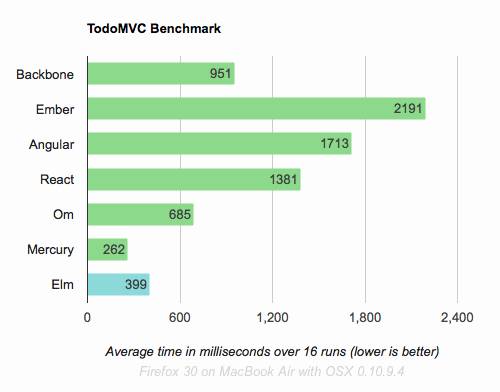
\includegraphics[width=1.0\textwidth]{images/virtual_dom.png}
    \caption{Geschwindigkeitsvergleich von TodoMVC-Implentierungen mit verschiedenen Frameworks \cite{elm}.}
    \label{fig:elm}
\end{figure}

Es ist zu sehen, dass Ember und AngularJS am langsamsten sind. Backbone ist in diesem Benchmark schneller als React.js, wobei die verwendete Implementierung der React.js-App nicht optimiert ist - Om\cite{om} kann als optimierte React-Version betrachtet werden, da Om im Grunde React mit nicht veränderbaren Datenstrukturen\footnote{Durch nicht veränderbare Datenstrukturen kann das diffing noch effizienter gestaltet werden, da viele Teilbäume nicht betrachtet werden müssen.} (immutable data-structures) ist. Backbone wie aber auch JQuery oder Dojo können theoretisch so schnell gemacht werden wie es möglich ist, dies ist aber so komplex, dass es nie gemacht wird und Wartbarkeit und Fehlervermeidung über Performance gestellt wird.
Die beiden schnellsten Frameworks benutzen ebenso eine virtual-DOM Implementierung und wie Om auch nicht veränderbare Datenstrukturen.
Dies ist auch der Grund weswegen immutable.js\citep{Immutable} verwendet wurde, da dies die render-Geschwindigkeit in den aufwändigsten Teilen verbessern konnte.

Ein weiterer Vorteil der virtuellen Darstellung ist die Unabhängigkeit des Browsers um die Applikation zu rendern, dass schlussendliche rendern des virtuellen DOMs in den richtigen DOM ist nicht zwingend. Es ist z.B. möglich den virtuellen DOM in ein Canvas-Element zu rendern oder ganz einfach in einen String. Durch das simple rendern zum String, was ganz ohne Browser möglich ist, beherrscht React.js isomorphes Rendering, d.h. die Inhalte können auf dem Server und im Client gerendert werden. So wird z.B. bei Instagram der erste Seitenaufruf auf dem Server alles weitere vom Clienten gerendert. Erste Versuche zeigen auch, dass man dies komplett agnostisch machen kann und alles kann auf Server/Client gerendert werden ohne das der Benutzer einen Unterschied merkt. So ist es denkbar das schwache Geräte mehr auf dem Server rendern und somit komplexe Inhalte vergleichsweise schnell darstellen können.

\subsubsection{Flux Architektur}

Flux ist die Applikations-Architektur die Facebook für ihre Frontend-Applikationen benutzt, es ergänzt React.js insoweit dass es einen unidirektionalen Datenfluss ermöglicht. Es ist wie eine alternative zu MVC zu verstehen und ist mehr ein Muster um Applikationen zu schreiben als ein Framework das einem rigoros die Struktur vorschreibt. Im Allgemeinen benutzt Flux das Paradigma der Datenfluss Programmierung\cite{johnston2004advances}, bei welchem ein Programm als gerichteter Graph modelliert wird. Typisch für das Paradigma ist die Benutzung eines Beobachter-Entwursfmuster wie z.B. eines pub/sub-System. Eine Auflistung und Bewertung typischer Muster ist zu finden unter \citep{signals}. Bei Flux wird für letzteres eine Abwandlung eines pub/sub-Systems benutzt.

Flux besitzt drei große Bestandteile: Einen Dispatcher, Stores und Views (React.js components). Desweiteren gibt es Actions, dies sind Hilfsmethoden vom Dispatcher und werden benutzt um eine semantische API zu unterstützen die alle Veränderungen die möglich sind in der Applikation beschreibt.

Das wichtigste Designziel von Flux ist der unidirektionale Datenfluss, wodurch die Logik deutlich verständlicher und nachvollziehbarer wird, siehe \ref{fig:flux}.

\begin{figure}[H]
    \centering
    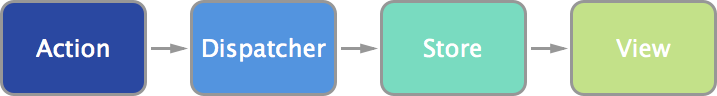
\includegraphics[width=1.0\textwidth]{images/flux.png}
    \caption{Dispatcher, Stores und Wiews sind unabhängige Knoten mit unterschiedlichen Ein und Ausgaben. Die Aktionen sind einfache Objekte die die neuen Daten enthalten und den Typ der Daten.}
    \label{fig:flux}
\end{figure}

\ref{fig:flux} zufolge ist es jedoch unmöglich dass eine Component den Zustand der Applikation verändern kann, was jedoch so gut wie immer nötig ist. Hier für werden die \textit{actions} benutzt, diese können von den Components benutzte werden um neue Daten an den Dispatcher zu schicken, welcher diese dann an den Store weiterleitet - welche dann die Darstellung der Component beeinflussen kann, siehe \ref{fig:flux_actions}.

\begin{figure}[H]
    \centering
    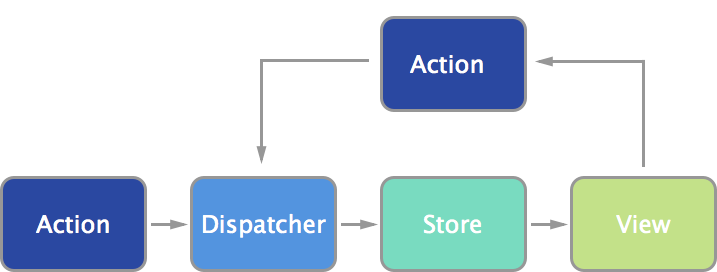
\includegraphics[width=1.0\textwidth]{images/flux_actions.png}
    \caption{Mithilfe von Actions ist die View in der Lage den Zustand der Applikation zu verändern.}
    \label{fig:flux_actions}
\end{figure}

Allem in allem ist die Facebook-Flux Architektur in Kombination mit React ein äußerst fortschrittlicher und zukunftssicherer Weg eine Webapplikation zu schreiben, womit die Anwendung dieser für die Erstellung der Enterprise-Infoboard eine gute Wahl erscheint.

\section{Architektur der Applikation}

Wie im vorherigen Abschnitt beschrieben wurde die Applikation mittels React und der Flux-Architektur realisiert. Anstelle der Flux-Bibliothek von Facebook wurde jedoch \textit{reflux} benutzt, reflux vereinfacht Flux insofern als das es keinen einzelnen Dispatcher benutzt, jede Action ist ihr eigener Dispatcher mit dem Ziel Flux eben mehr zu vereinfachen und unnötigen Quelltext (sogennanten Boilerplate) zu reduzieren\footnote{Keinen zentralen Dispatcher zu benutzen hat auch Nachteile, für dieses Projekt waren die jedoch nicht von Relevanz.}. Eine Vollständige Erklärung für reflux ist auf dem Blog des Autors zu finden unter \cite{reflux}. reflux ist nicht der einzige Versuch eine alternative bereitzustellen, mittlerweile gibt es über 10 verschiedene Flux-Bibliotheken\footnote{Ein Vergleich dieser ist hier zu finden \url{https://github.com/voronianski/flux-comparison}} - mit teilweise großen Gemeinden dahinter oder Firmen wie z.B. \textit{Yahoo} mit \textit{Fluxible}. Der Funktionsinhalt der verschiedenen Flux-Bibliotheken ist mehr oder minder gleich, somit könnte reflux mit Leichtigkeit ausgetauscht werden, wenn es denn nötig wäre.
Die Entwicklung in diesem Bereich ist jedoch äußerst spannend und hat zum Zeitpunkt dieser Arbeit mit redux ihren Höhepunkt gefunden \citep{redux}, wo die Stores gar keinen State mehr besitzen und nur noch als Action-Aggregatoren dienen. Dies ermöglicht das der Zustand der Applikation vor- und zurückgespult werden kann, er ist ja rein von den gesendeten Actions abhängig.

\subsection{Überblick}

\begin{figure}[H]
    \centering
    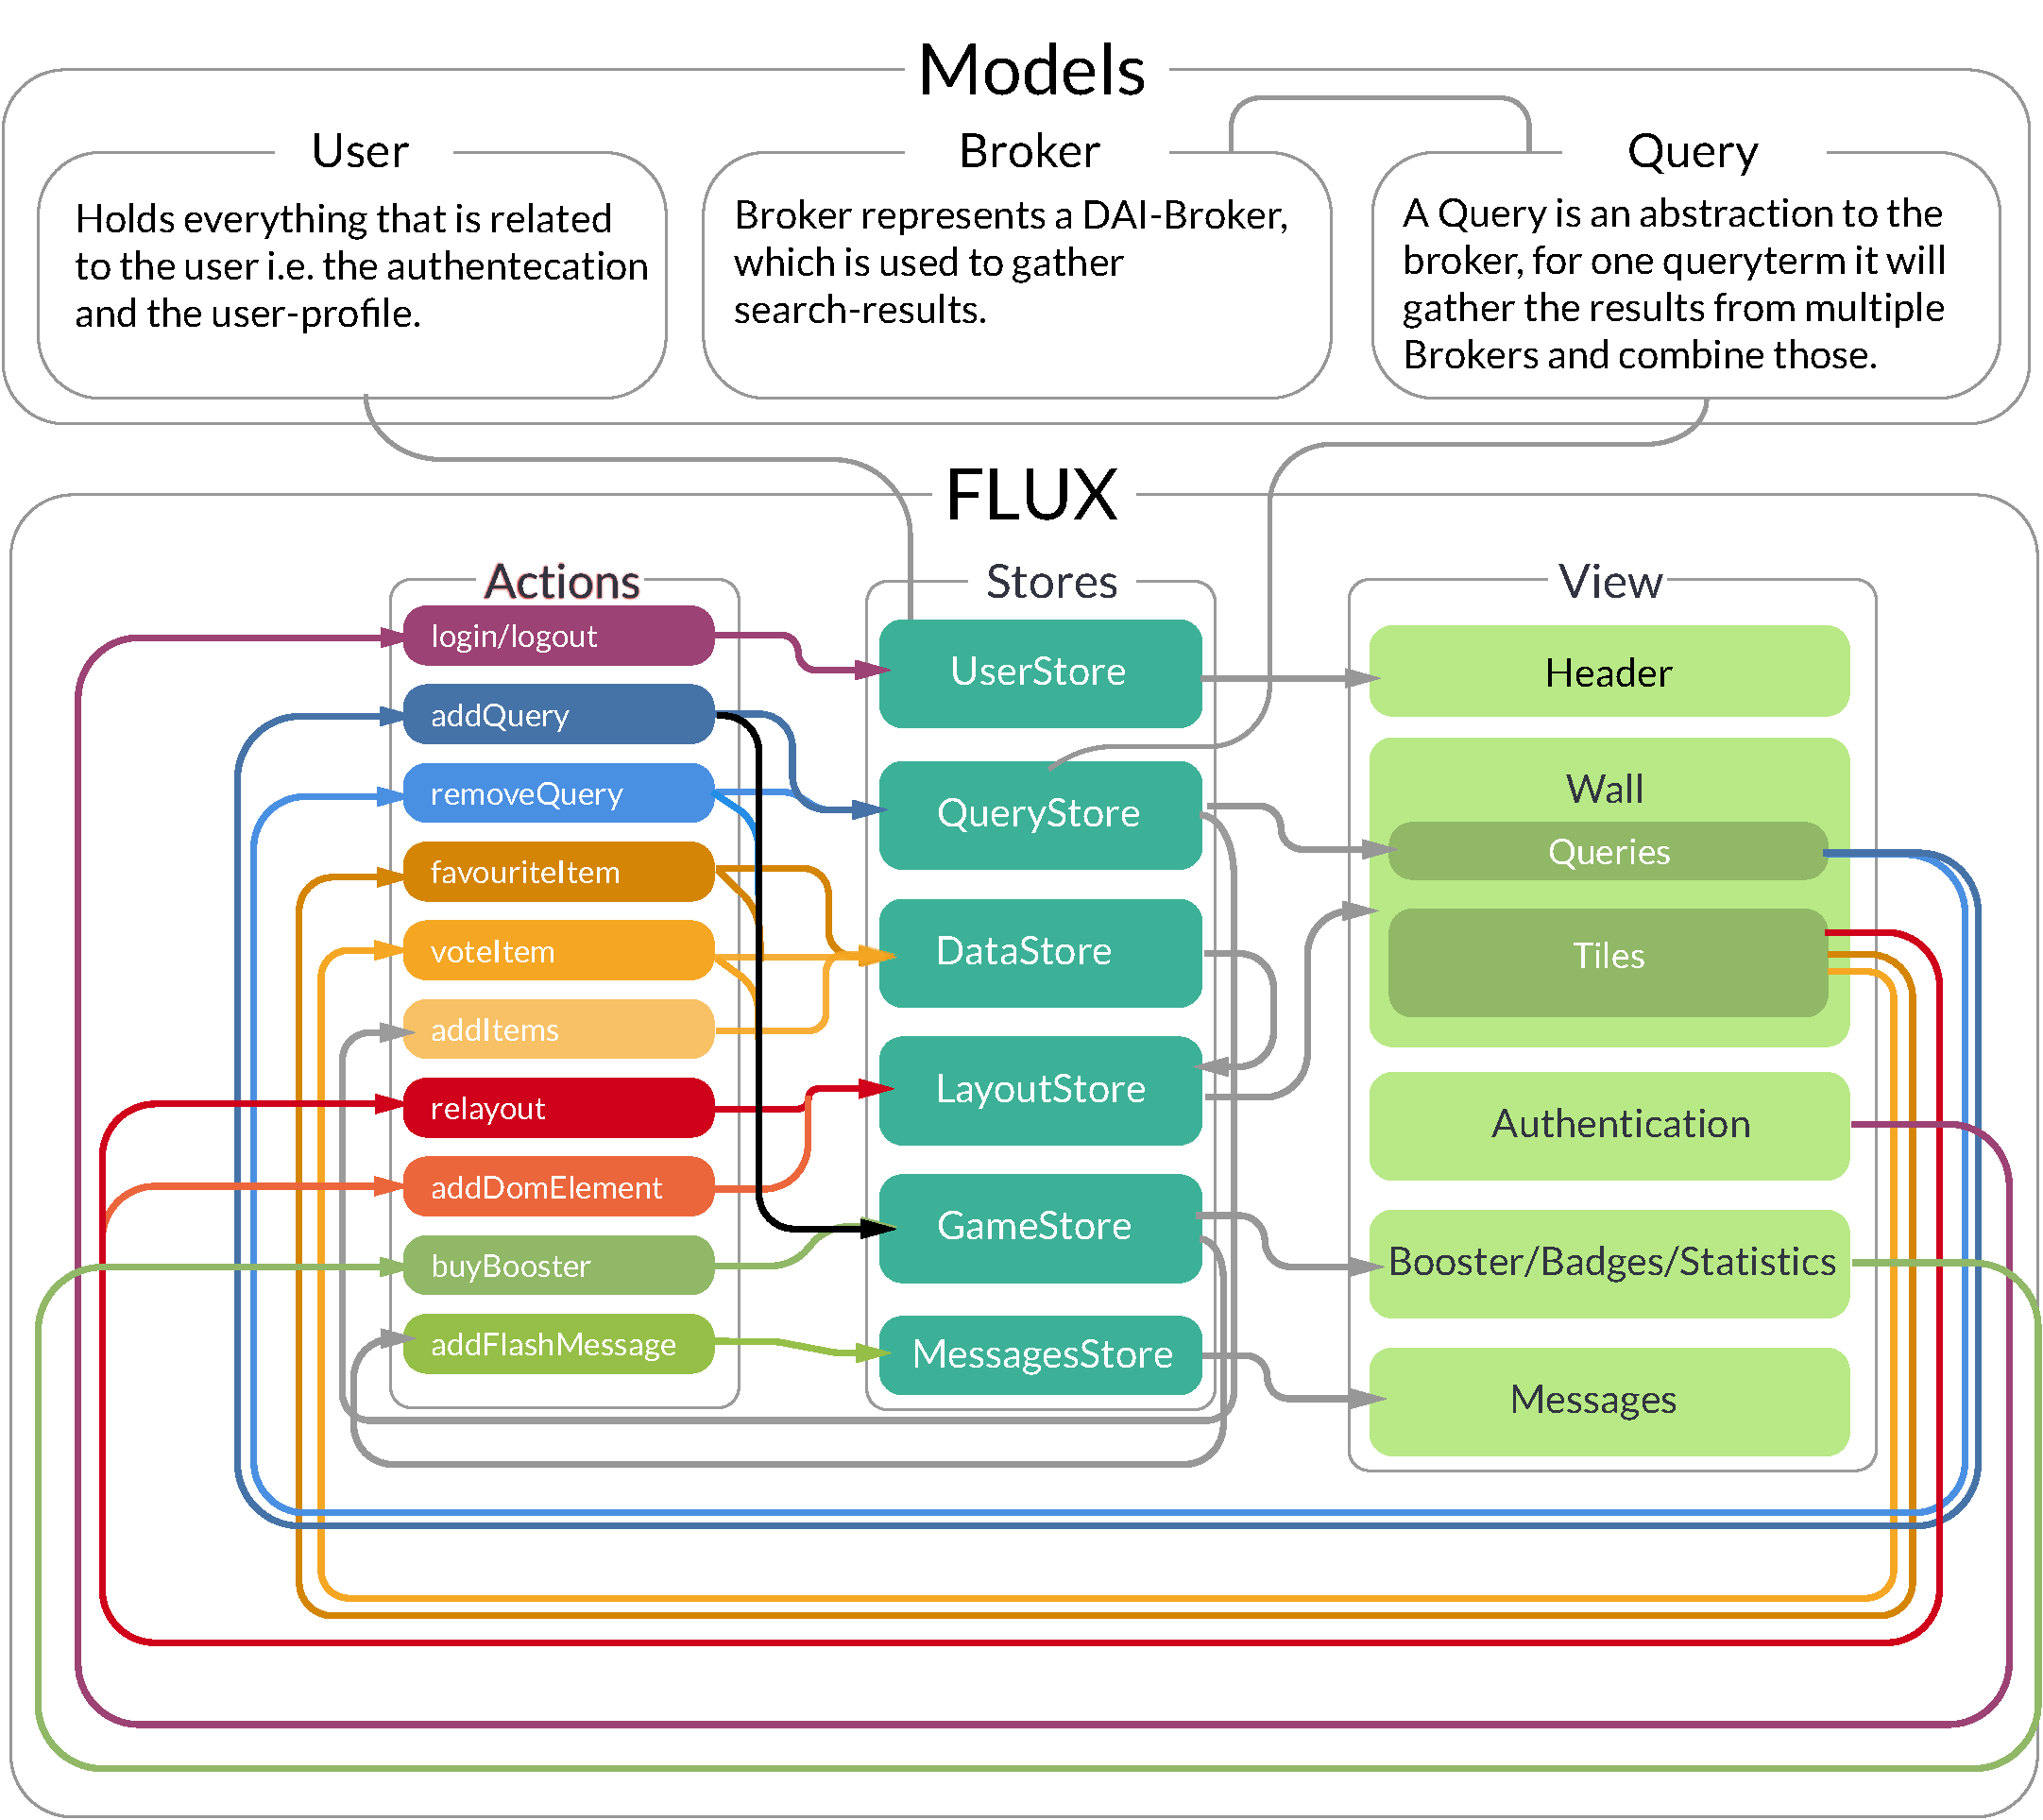
\includegraphics[width=1.0\textwidth]{images/architecture.pdf}
    \caption{Die wichtigsten Bestandteile der Applikation.}
    \label{fig:architecture}
\end{figure}

Die Abbildung \ref{fig:architecture} zeigt einen Überblick über die gesamte Architektur, sie wurde bewusst nicht in einem Klassendiagramm dargestellt da die Applikation keinen Strengen Objektorientierten Stil verfolgt und das Schaubild nicht sonderlich zum Verständnis beitragen würde. Dies ist eine grobe Abstraktion, doch reicht diese Abbildung um sich im Quelltext zurecht zu finden.

Es ist deutlich zu sehen das der komplette Datenfluss bzw. Programmfluss mittels der Flux-Architektur modelliert wurde, was daran zu erkennen ist dass jegliche Interaktionen der View werden mittels Actions an die jeweiligen Stores weitergegeben wird die dann den neuen Zustand an die View abermals weitergeben.

Zu Flux gibt es noch drei Klassen die von den jeweiligen Stores benutzt werden, die Auslagerung dieser Logik in eigene Klassen dient der Übersichtlichkeit, verdeutlicht jedoch auch dass alle Komponenten mit denen der Benutzer nicht direkt interagiert nicht Teil des Flux-Datenflusses sein müssen.

Im folgenden werde ich genauer auf die Stores eingehen.

\subsection{Stores}

Die Stores sind zuständig den Datenfluss zu verwalten, insgesamt enthält die Applikation 6 Stores: \texttt{UserStore}, \texttt{QueryStore}, \texttt{DataStore}, \texttt{LayoutStore}, \texttt{GameStore} und \texttt{MessagesStore}.
Der \texttt{UserStore} und \texttt{MessagesStore} sind jedoch äußerst trivial und sind nur wenige Zeilen lang. Die wichtigsten sind die anderen 4, diese werde ich nun im Detail behandeln.

\subsubsection{QueryStore}

Der \texttt{QueryStore} abonniert die Aktionen \texttt{addQuery} und \texttt{removeQuery}, er abstrahiert die Anfrage an die \texttt{Broker} d.h. für jeden Suchbegriff werden alle verfügbaren \texttt{Broker} angefragt, nach jeder Antwort eines Brokers wird die Nachricht \texttt{addItems} mit den Ergebnissen gesendet. Auf diese Nachricht hört der \texttt{DataStore}.

\subsubsection{GameStore}

Der \texttt{GameStore} liefert alles was für die Verspielisierung der Applikation relevant ist - wie die Bereitstellung der Punkte, der Bestenlisten und Trophäen aller Benutzer der Applikation. Weiterhin abonniert er alle Aktionen auf denen Punkte definiert sind wie das bewerten eines Suchergebnisses und sorgt dafür dass diese Aktionen vom Backend verarbeitet werden.

Um den sozialen Faktor zu erhöhen reagiert der \texttt{GameStore} ebenfalls auf alle Aktionen aller anderen Benutzer, dies geschieht quasi in Echtzeit und sorgt dadurch z.B. für eine äußert lebendige Statistikseite (auf dieser werden die Daten aller Benutzer angezeigt).
Damit das ganze noch effizient bleibt wurden WebSockets verwendet die deutlich weniger ``Overhead'' besitzen als normale HTTP-requests.

\subsubsection{DataStore}

Der \texttt{DataStore} stellt alle Daten bereit die für die Darstellung benötigt werden, dies sind die Suchergebnisse die mit dem Profil des Benutzers verbunden werden um anzuzeigen welche Ergebnisse bewertet/favorisiert wurden und die Suchanfragen, die zur Laufzeit verändert werden können. Herausforderungen hier waren es Duplikate in den Suchergebnissen zu verarbeiten und die Interaktion mit den Suchergebnissen.

Hierzu hört er auf die Nachricht \texttt{addItems} welche eine Liste mit Suchergebnissen enthält. Diese Daten sind noch ganz ohne die Bewertungsdaten, welche hier angefragt werden und in die Suchergebnisse integriert werden. Sobald das geschehen ist, wird allen Abonnenten (in dem Fall der \texttt{LayoutStore} mitgeteilt dass der Datensatz sich verändert hat. 

Eine Besonderheit ist die Benutzung einer nicht veränderbaren \texttt{OrderedMap} in welcher die Suchergebnisse mit ihrer URL als Schlüssel gespeichert sind. Die Suchergebnisse werden in der Applikation noch viel weitergereicht weswegen viele Fehler vorgebeugt werden da nur der \texttt{DataStore} selbst die Suchergebnisse verändern kann.

\subsubsection{LayoutStore}

Im Design-Abschnitt wurde lange darauf eingegangen was die Layouting-Engine alles können muss, leider konnte keine der OpenSource-Bibliotheken allen Anforderungen gerecht werden. Deswegen wurde extra für die Darstellung eine eigene Layouting-Engine erstellt.
Die Grundlage ist die absolute Positionierung innerhalb des Browsers, diese ist notwendig um Animationen zu ermöglichen. Es gibt verschiedene Arten DOM-Elemente mittels CSS zu positionieren:

\begin{enumerate}
  \item Mithilfe von \texttt{top/left}.\\
  \begin{minted}{css}
  .position-top-left {
      position: absolute; /* or relative/fixed */
      top:  50px;
      left: 50px;
  }
  \end{minted}
  \item Mithilfe von \texttt{transform: translate(x, y)}. Dies ist allgemein anerkannt schneller als zu sein und hat den Vorteil das subpixel-animationen möglich sind was im Allgemeinen flüssigere Animationen erlaubt. \\
  \begin{minted}{css}
  .position-translate {
      position: absolute; /* or relative/fixed */
      transform:         translate(50px, 50px);
      -webkit-transform: translate(50px, 50px);
  }
  \end{minted}
  \item Mithilfe von \texttt{transform: translate3D(x, y, z)}. Dies ist mit Abstand das schnellste. Hierbei werden die Elemente zu Texturen gerendert und mit Einsatz des Grafikprozessors animiert. Dadurch ist es sogar möglich auf mobilen Endgeräten flüssige Animationen zu haben, da diese meist dedidizierte Grafikprozessoren haben.
  \begin{minted}{css}
  .position-translate3D {
      position: absolute; /* or relative/fixed */
      transform:         translate3D(50px, 50px);
      -webkit-transform: translate3D(50px, 50px);
  }
  \end{minted}
  \texttt{transform3D} wird von allen aktuellen Browsern soweit unterstützt das unser Szenario möglich ist\cite{transform3d}. Was weiterhin zu beachten ist, dass am Ende immer gerundete Pixelwerte innerhalb von \textsc{translate3D(x, y, z)} benutzt werden sollten. Da Ansonsten die Elemente unscharf sind, siehe \ref{fig:blurry}.

\begin{figure}[H]
	\centering
	
\includegraphics[width=1.0\textwidth]{images/blurry_tiles.png}
	\caption{Links eine Kachel mit geraden Werten bei \texttt{translate3D}, rechts mit jeweils $.5$ bei $x/y$.}
	\label{fig:blurry}
\end{figure}

\end{enumerate}

Es ist eine Grundanforderung Geräte mit unterschiedlich großen Bildschirmen zu unterstützen, was dadurch erzielt wird, dass die die Anzahl der Spalten variabel ist.
Es gibt zwei Möglichkeiten die Anzahl der Spalten variabel zu machen:

\begin{enumerate}
  \item Berechne die Breite mittels Javascript bevor das Element in den DOM eingefügt wird und setze die Breite mittels CSS.
  \item Durch die Benutzung von \textit{Media Queries} können in CSS verschiedene Darstellungen für unterschiedliche Bildschirmbreiten beschrieben werden.
\end{enumerate}

Für die Positionierung müssen wir wissen wie viele Spalten zu jedem Zeitpunkt dargestellt werden sollen. Dafür muss die Breite in Javascript berechnet werden, somit liegt 1. nahe. Versuche haben jedoch gezeigt, dass es schneller ist die Breite des Elementes nicht per Javascript zu setzen sondern diese über die \texttt{Media Queries} zu bestimmen. Zwar bedeutet dies, dass die gleiche Logik an zwei Orten in 2 Sprachen steht, aber da dies nicht mehr als jeweils 10 Zeilen sind ist es für die resultierende bessere Geschwindigkeit hinnehmbar.

Die Breite aller Elemente ist zu jedem Zeitpunkt gleich, die Höhe ist jedoch variabel. Da es unmöglich ist die Höhe auszurechnen ohne eine komplette Browser-Engine zu implementieren, muss das Element in den DOM eingefügt werden bevor wir dessen korrekte y-Position berechnen können, hierfür existiert die Aktion \texttt{addDOMElement}, welche die gleichnamige Funktion im \texttt{LayoutStore} ausführt. Diese Funktion ist neben der \texttt{relayout}-Funktion der einzige Ort an dem der DOM direkt ausgelesen wird, nämlich die Höhe des Elementes mit \texttt{offsetHeight}. Solange kein \texttt{resize}-Event getriggert wird müssen wir diesen Wert auch nicht ein zweites mal auslesen.
Wenn zu allen Suchergebnissen eine Kachel angelegt wurde, wird die \texttt{layout}-Funktion aufgerufen und die Kacheln bewegen sich auf dem Bildschirm.

Der vollständige Programmfluss ist komplex, da er sehr auf Geschwindigkeit getrimmt wurde, der Programmteil ist ausführlich kommentiert und beschrieben.

Allgemein hat die Flux-Architektur hier gut funktioniert, der größte Manko entstand beim Abgleichen des LayoutStores mit dem \texttt{DataStore}. Wenn nun ein Element positiv bewertet wird, muss das Layout neu berechnet werden. Der LayoutStore weiß inhärent jedoch nicht welches Element sich verändert hat, es muss durch alle Elemente des \texttt{DataStores} mit den eigenen abgleichen. Dies fühlt sich nicht optimal an, jedoch ist stellt sich die Frage auf ob mit einer anderen Architektur das Problem einfacher wäre.

\subsection{Views}

Als View wird das Interface bezeichnet mit dem der Benutzer schlussendlich interagieren kann. Für jede View wird React und React-Bootstrap verwendet, die Gründe warum React verwendet wird sind in \ref{sec:flux} genauer ausgeführt.

\subsubsection{Responsives Design}

Responsives Webdesign bezeichnet ein Paradigma bei dem Webseiten daraufhin geschrieben werden, dass sie Inhalte auf unterschiedliche Endgeräte optimieren, was praktikabel bedeutet das Inhalte abhängig von der Bildschirmbreite des Gerätes angezeigt werden.

Aktuell wird dies so umgesetzt dass jeglicher Inhalt mit der Benutzung eines \textit{Grid}-Systems dargestellt wird.

\begin{quote}
	Grid systems are used for creating page layouts through a series of rows and columns that house your content.
\end{quote}

Damit wird auf der Webseite von Bootstrap \cite{bootstrap} das Grid-System erklärt, für mehr Informationen wie genau Grid-Systeme funktionieren siehe dort.
In dieser Applikation wird das von Bootstrap bereitgestellte Grid intensiv benutzt um auf jedem Endgerät eine möglichst gute Benutzererfahrung zu garantieren. 

\subsubsection{Erstellte React-Komponenten}

Wie auch in anderen Interface-Bibliotheken wird in React das Interface in Komponenten unterteilt (in anderen Bibliotheken auch \textit{widgets} gennant).

Jede React-Komponente besitzt Lebenszyklus-Methoden, welche eine Feingranule Benutzung der Komponenten ermöglicht \cite{lifecycle}.
Eine Benutzung dieser ist jedoch komplett optional, die einfachste React-Komponente hat nur einer \texttt{render}-Methode. An dieser Stelle wurde überlegt eine Einführung für React zu schreiben, stattdessen verweise ich auf externe Tutorials wie das offizielle von Facebook\cite{tutorial}.

Es wurden ca. 30 React-Komponenten erstellt, viele davon wurden an mehreren Stellen der Applikation verwendet. Unterteilt sind sie semantisch nach Aufgabe/Seiten wie z.B. \texttt{settings}, \texttt{stats} oder \texttt{utility}.
Eine Minimalübersicht findet sich in \ref{fig:architecture}, in welchem Alle Komponenten gezeigt werden die Teil des Flux-Kreises sind, alle restlichen sind statisch und spielen für die Architektur keine Rolle.

Die erstellten Seiten sind in , \ref{fig:booster}, \ref{fig:settings}, \ref{fig:actions} zu sehen, \ref{fig:badges}.


Die wichtigste Seite ist die mit der eigentlichen Applikation, nämlich der Suchmaschine, zu sehen in \ref{fig:wall}. Der Benutzer wird sich vorraussichtlich die meiste Zeit auf dieser Seite befinden, deshalb sind auch alle relevanten Aktionen, neben dem einloggen und Booster kaufen), nur auf dieser Seite möglich. Für weitere Details zu dem Konzept dieser Seite siehe \ref{chap:concept:wall}.

\begin{figure}[H]
    \centering
    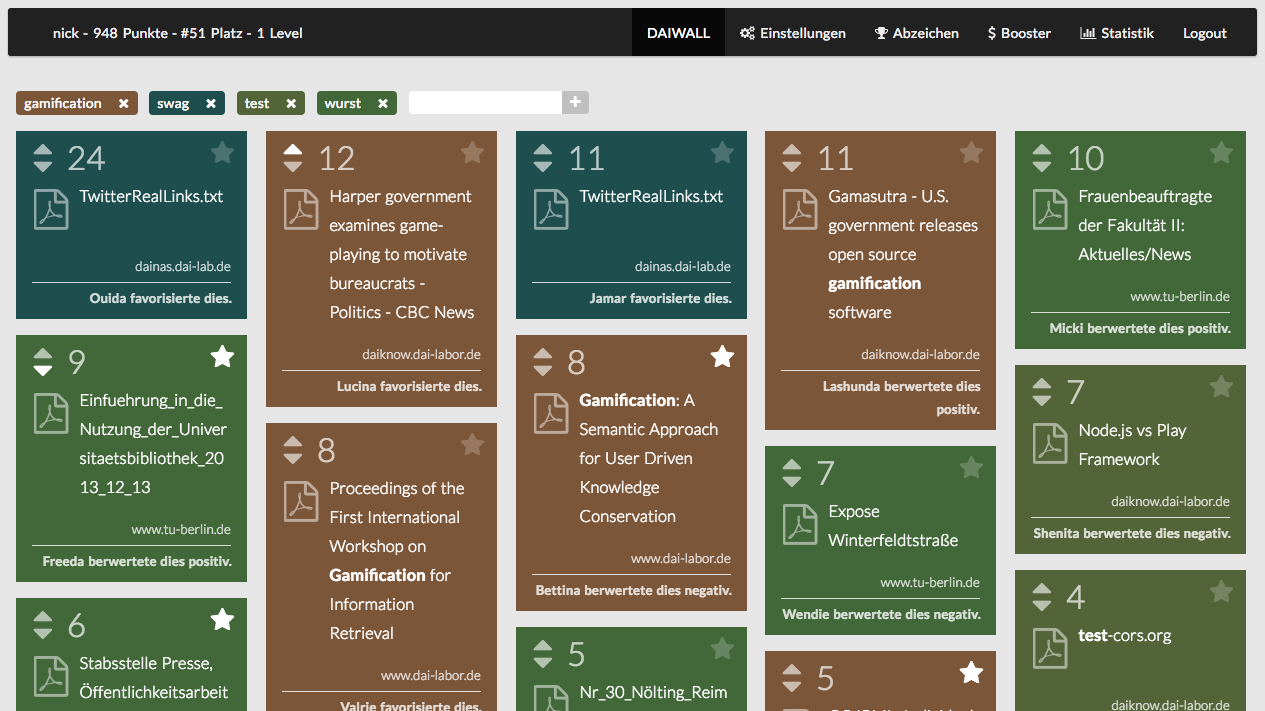
\includegraphics[width=0.9\textwidth]{images/infoboard_wall.png}
    \caption{Dies ist die Hauptapplikation, hier kann der Benutzer nach verschiedenen Begriffen suchen, die Suchergebnisse Bewerten/Favorisieren und sehen wer welche Aktion als letztes auf ein Suchergebnis ausgeführt hat.}
    \label{fig:booster}
\end{figure}

Neben der Seite mit der Suchmaschine, sind noch 4 weitere Seiten verfügbar. Diese dienen hauptsächlich der Gamification. Für den Nutzer am interessantesten ist die Seite mit den Benutzerstatistiken, zu sehen in \ref{fig:usersite}.
Weiterhin gibt es noch die Seite auf dem der Benutzer den derzeitigen Status seines aktuellen Boosters sehen kann und falls er keinen hat, die Möglichkeit besitzt einen neuen Booster zu erwerben, siehe \ref{fig:booster}. Einstellungen, wie das Auswählen des Farbschemas kann der Nutzer ebenfalls auf einer dedizierten Seite tätigen, siehe \ref{fig:settings}.

\begin{figure}[H]
    \centering
    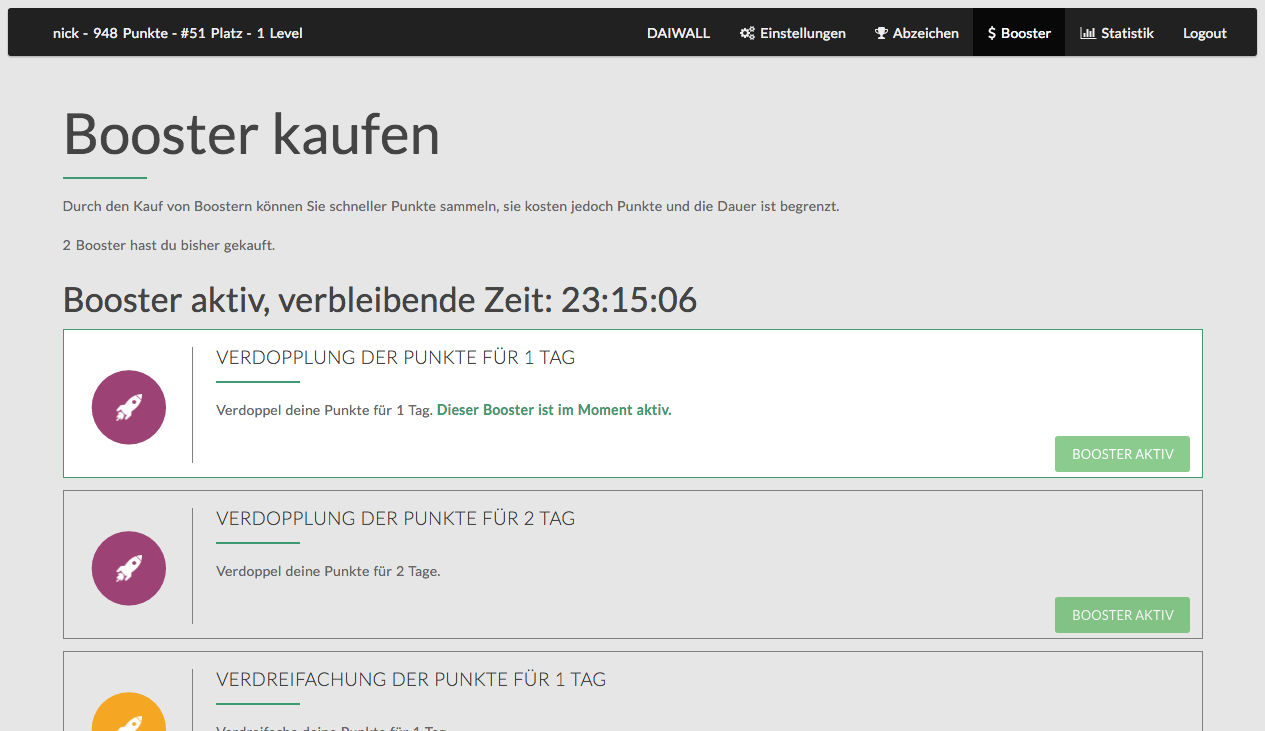
\includegraphics[width=0.9\textwidth]{images/infoboard_booster.png}
    \caption{Auf dieser Seite kann der Benutzer verschiedene Booster erwerben und sehen wie lange der aktuelle noch aktiv ist.}
    \label{fig:booster}
\end{figure}

\begin{figure}[H]
    \centering
    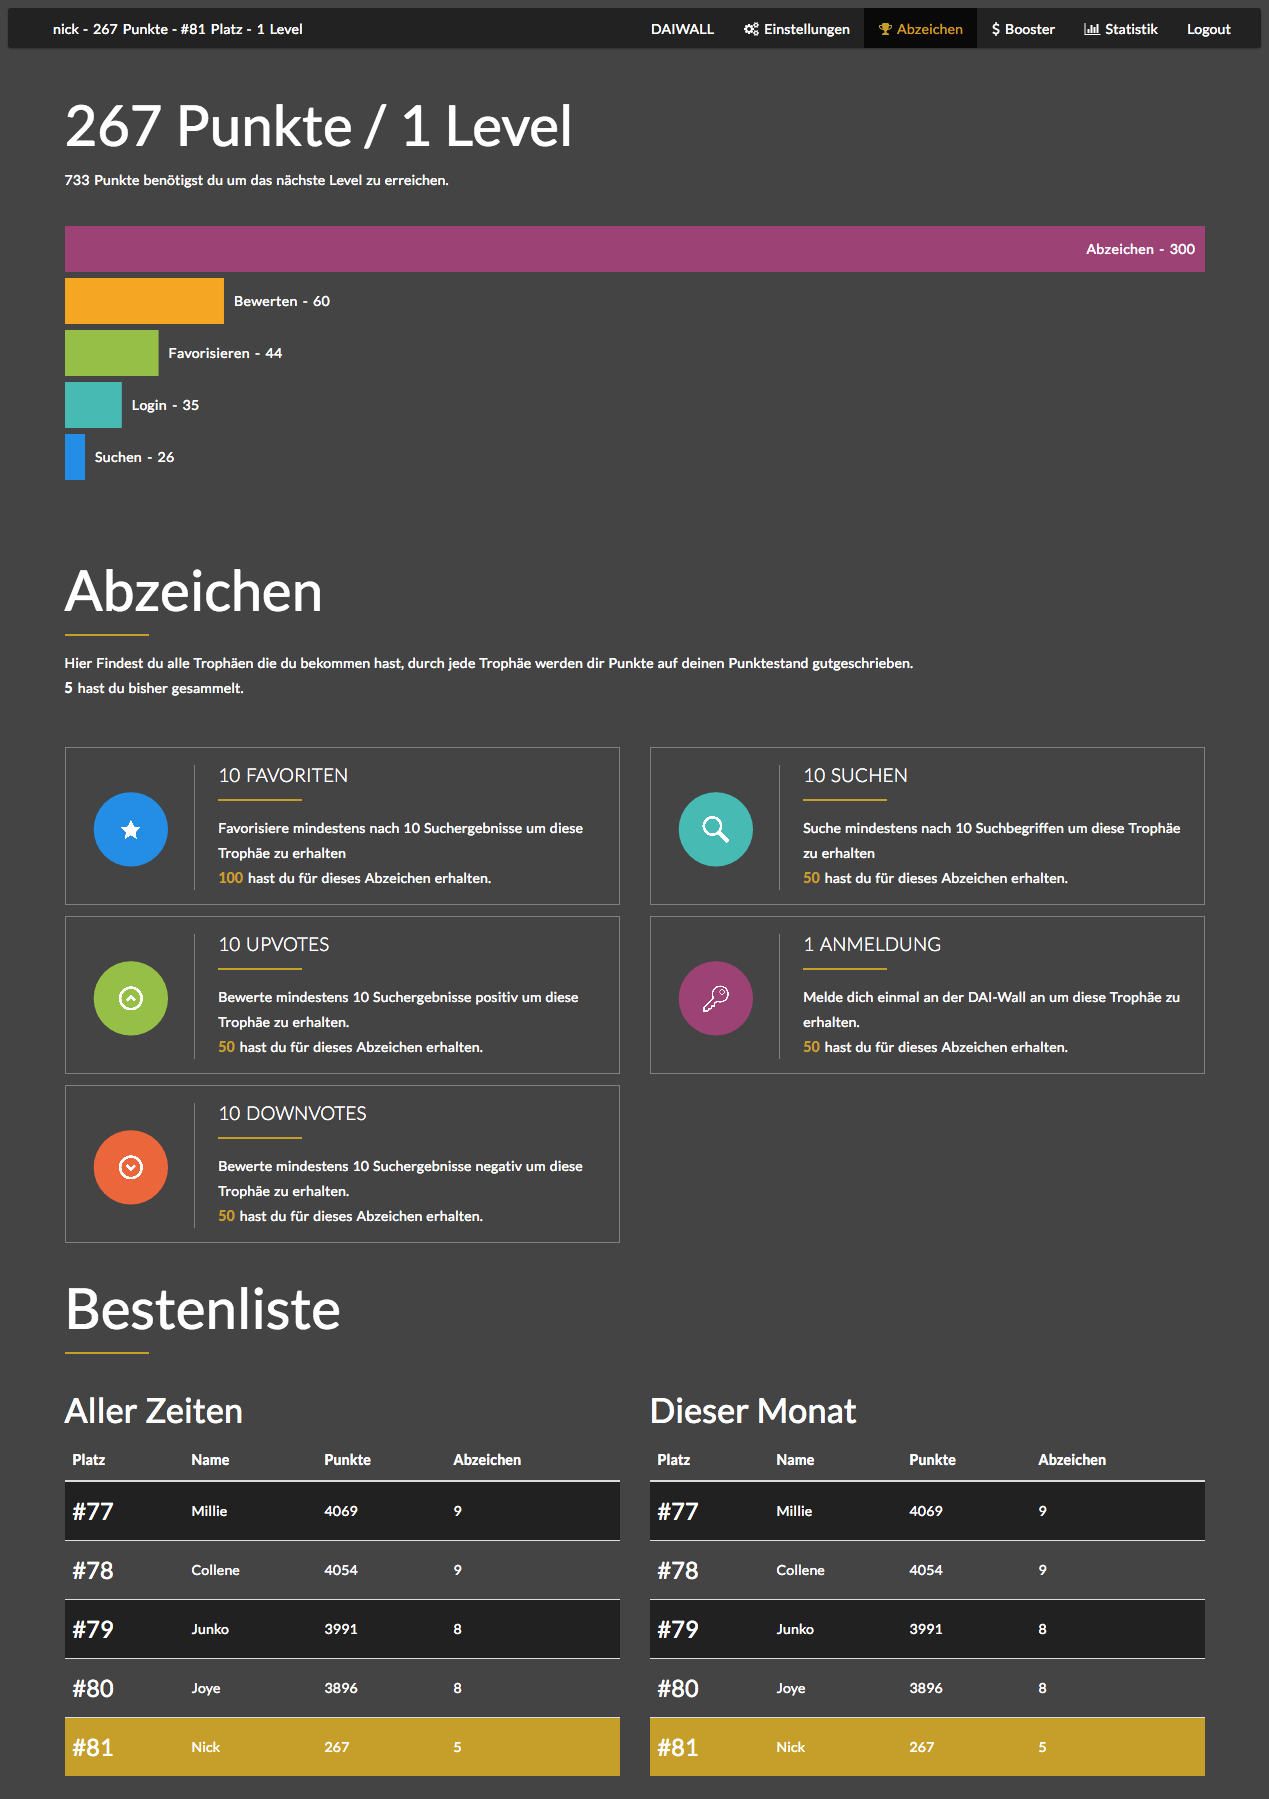
\includegraphics[width=0.9\textwidth]{images/infoboard_usersite.png}
    \caption{Auf dieser Seite kann der Benutzer einsehen wie viele Punkte er hat, wie sie aufgeteilt sind, welche Abzeichen er besitzt und welche Personen um ihm auf der Bestenliste sind. }
    \label{fig:usersite}
\end{figure}

\begin{figure}[H]
    \centering
    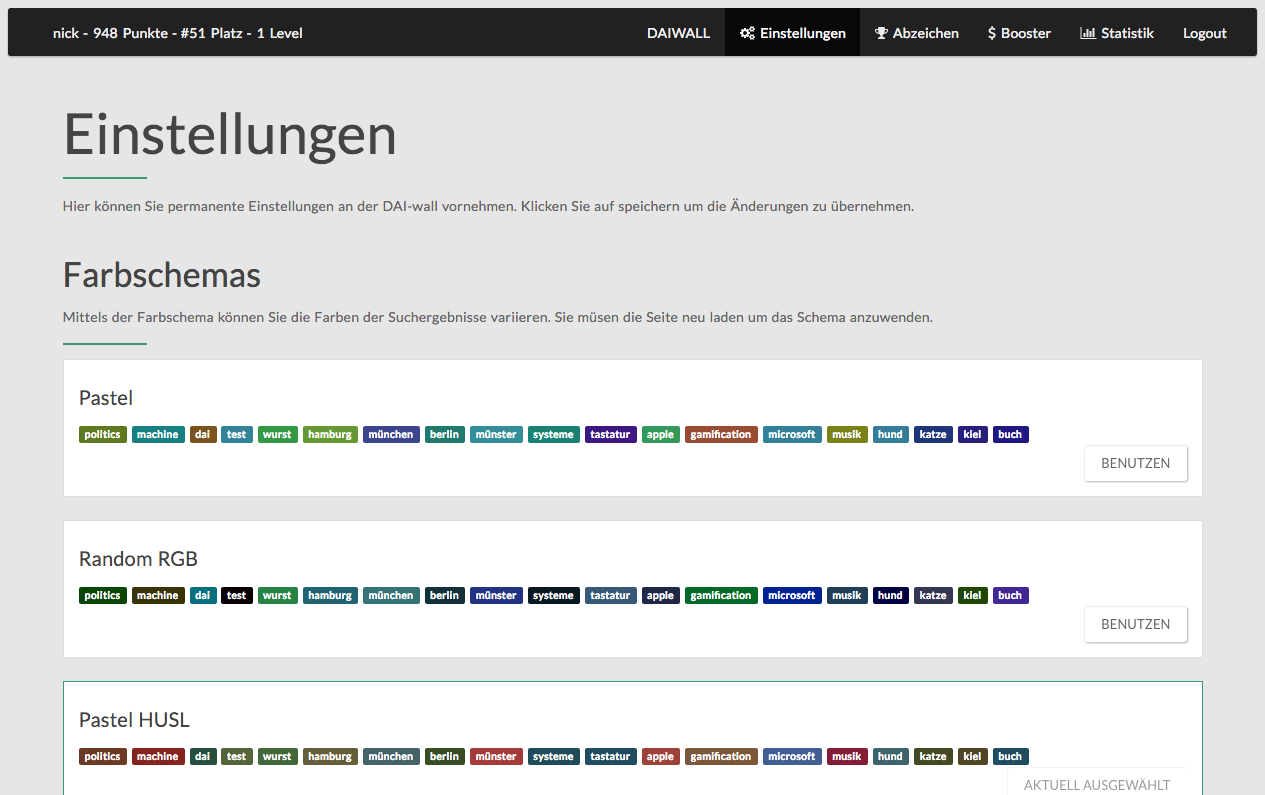
\includegraphics[width=0.9\textwidth]{images/infoboard_settings.png}
    \caption{Auf dieser Seite kann der Benutzer einsehen wie viele Punkte er hat, wie sie aufgeteilt sind, welche Abzeichen er besitzt und welche Personen um ihm auf der Bestenliste sind.}
    \label{fig:settings}
\end{figure}

Eine allgemeine Übersicht der Aktivität aller Nutzer ist auf der Statistik-Seite zu sehen. Diese Seite ist dafür gedacht auf einem Fernseher, der in einem öffentlichen Raum des Betriebes aufgehängt ist, angezeigt zu werden. Die Seite unterteilt sich in drei Abschnitte. Der erste Teil zeigt zwei Bestenlisten an, eine für den kompletten Zeitraum und eine für den letzten Monat. Im zweiten Teil ist die Gesamtpunktzahl der Mitarbeiter zu sehen, wie auf der Seite mit den Benutzerstatistiken aufgeteilt in die einzelnen Kategorien. Der Dritte Teil besteht aus einem Livestream der Nutzeraktivitäten, jedes mal wenn z.B. eine Aktion ausgeführt wurde wird dies dort angezeigt. Die Seite ist zu sehen in \ref{fig:stats}.


\begin{figure}[H]
    \centering
    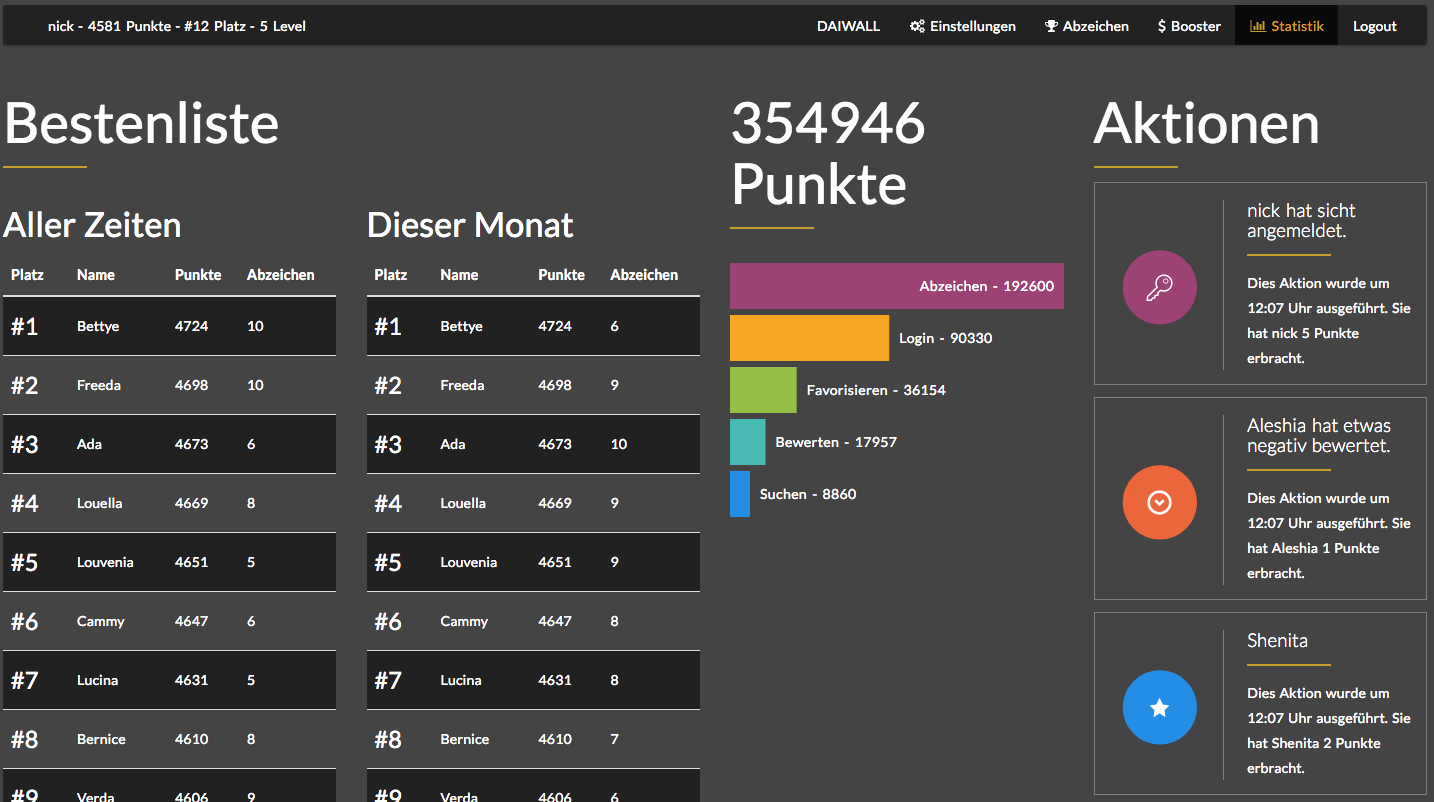
\includegraphics[width=0.9\textwidth]{images/infoboard_stats.png}
    \caption{Die Gesamtstatistikseite. Um den Effekt der Gamification zu erhöhen, sollte diese an einem öffentlichen Ort des Betriebs permanent gezeigt werden.}
    \label{fig:stats}
\end{figure}


Der Aufbau der eigentlichen Komponenten wird Beispielhaft in \ref{chap:appendix:component} anhand der \texttt{Query}-Komponente gezeigt.

\section{Backend}\label{sec:backend}

Im Verlaufe der Arbeit wurde erkannt das eine dedizierte Backend-Applikation nötig ist um den Grad der Interaktion und Dynamik zu ermöglichen die als Ziel gesetzt wurde. Es gibt einige Frameworks die zur Frage standen, aber schließlich viel fiel die Entscheidung auf node.js, da dadurch die Möglichkeit  bestand einiges an Code mit dem Frontend zu teilen. Das node.js \textit{non-blocking} ist und \textit{event-driven IO} benutzt macht es Vorteilhaft für Applikation die viele Anfragen verarbeiten werden müssen. Anders als in klassischen Frameworks wie rails oder django wo bei jedem request ein neuer Thread aufgemacht der solange blockiert ist bis er abgehandelt ist, wird jede Anfrage von einem \textit{event-loop} abgehandelt \citep{tilkov2010node}. Alles in node.js ist asynchron, weswegen diese Anfragen nicht blockieren. Damit ist es mit node.js z.B> möglich bis zu 1 Million gleichzeitige Verbindungen zu halten \cite{node1m}.

Als Datenbank wurde mysql verwendet, die mittels einem Object Relationship Mapper (kurz ORM) angesteuert wird. Mit einem ORM ist es möglich Datenbanken mittels Klassen und Objekten zu abstrahieren. ORM ist jedoch nur eine einfach Abstraktion und beherrscht nicht alles was SQL kann, jedoch reichen die Fähigkeiten des ORMs meistens aus und es kann immer auf rohes-SQL zurückgeriffen werden. Das Verwendete ORM ist sequelize \cite{sequelize}. Mysql ist auf den Systemen des DAI schon installiert, ohne Einschränkung kann z.B. auch sqlite oder Postgres benutzt werden.

Das verwendete Datenmodell kann in \ref{fig:database} betrachtet werden, es ist komplett mit sequelize beschrieben und ist damit ohne viel Aufwand veränderbar.

\begin{figure}[H]
	\centering
	\includegraphics[width=0.65\textwidth]{images/database}
	\caption{Das benutzte Datenmodell der Applikation. Ein Item ist ein Suchergebnis, ein Vote eine Bewertung, und eine Action alle vom Benutzer ausgeführten Aktionen.}
	\label{fig:database}
\end{figure}

\subsection{HTTP-API}

Die Kommunikation von Backend und Frontend geschieht per HTTP-Anfragen, das verwendete Framework ist express.js, es wurde überlegt ein API-Framework wie Swagger zu benutzen. Diese erstellen eine einheitliche, sich selbst-aktualisierende Dokumentation wie auch Tests \cite{haupt2014model}.
Damit wäre jedoch eine weitere Technologie eingeführt worden und da sich die Anzahl der Endpunkte nur auf 8 beläuft, haben wir uns bewusst dagegen entschieden. Im folgenden wird Schemenhaft der Ablauf der Anfragen aller Endpunkte illustriert.

\begin{description}
	\item[\texttt{POST  /user/action}] Jede Aktion des Benutzers wird an diesen Endpunkt gesendet der folgenden Ablauf besitzt: 
	\begin{enumerate}
		\item Finde den angegebenen Benutzer in der Datenbank
		\item Suche alle Booster des Benutzers und finde heraus ob einer aktiv ist
		\item Füge die Aktion in die Datenbank ein, wenn ein Booster aktiv ist, multipliziere die Punkte der Aktion mit dessen Multiplikator
		\item Falls die Aktion auf einem Suchergebnis statt fand, verknüpfe dieses mit der Aktion
		\item Berechne die Abzeichen neu, wenn sich diese von den bisherigen Abzeichen unterscheiden, füge die neuen in die Datenbank ein und füge sie der Antwort hinzu
		\item Antworte mit der erstellten Aktion und ggf. mit den erstellten Abzeichen
	\end{enumerate}
	\item[\texttt{POST /user/vote}] Sobald der Benutzer ein Suchergebnis bewertet, wird diese Anfrage gesendet. Der folgende Ablauf findet statt:
	\begin{enumerate}
		\item Finde den angegebenen Benutzer in der Datenbank
		\item Finde das angegebene Suchergebnis in der Datenbank und erstelle es neu falls nicht vorhanden.
		\item Finde die bisherige Bewertung des Suchergebnissen oder erstelle diese neu falls nicht vorhanden.
		\item Setze den neuen Wert für die Bewertung und speichere diese
		\item Antworte mit der erstellten Antwort
	\end{enumerate}
	\item[\texttt{POST /user/booster}] Sobald der Benutzer einen Booster erwirbt wird mittels dieser Anfrage die Transaktion in der Datenbank festgehalten. Dazu wird der angegebene Benutzer gesucht und der gekaufte Booster erstellt.
	\item[\texttt{GET /points}] Diese Anfrage nimmt zwei Parameter, Anfangsdatum und Enddatum. Das Ergebnis ist eine Liste aller Benutzer mit ihren jeweiligen Punkten und Abzeichen, zusätzlich werden die Punkte aller Nutzer Kategorieunterteilt und komplett aufsummiert zurückgeliefert.
	\item[\texttt{GET /items}] Diese Anfrage nimmt als Parameter eine Liste an Suchergebnissen-URLs und findet alle Bewertungen und Aktionen auf das Suchergebnis zeigen. Die Bewertungen werden aufsummiert.
	\item[\texttt{GET /actions}] Diese Anfrage liefert die letzten 50 Aktionen zurück.
	
\end{description}

\subsection{Websockt-API}

Um die Dynamik des Infoboards zu maximieren wurden Websockets verwendet die auf alle ausgeführten Aktionen des Systems reagieren und dadurch z.B. die Gesamtpunktzahl erhöhen. Websockets wurden jedoch nicht in ihrer reinen Form benutzt, sondern mittels der Bibliothek socket.io \cite{rauch2013socket}. Diese ermöglicht neben einer einfacheren Benutzung von Websockets, 
auch einen Alternativmodus mittels polling um Geräte zu unterstützen die keine Websockets besitzen.


\chapter{Fazit und Ausblick}

In dieser Arbeit wurde vieles gemacht das vor wenigen Jahren noch nicht möglich gewesen wäre, die gewählten Technologien sind größtenteils jung und die Anwendung war, trotz großer Firmen die dahinter stehen, gewagt. Das Entwickeln der Applikation war damit zu einem gewissen Teil eine Fallstudie für neue Technologien in der Webentwicklung.
Rein technologisch betrachten ist die Arbeit jedoch ein voller Erfolg, sie ist performant, ästhetisch anspruchsvoll (Dies ist natürlich subjektiv) und die unidirektionale Architektur übersichtlich und erweiterbar.
Wenn man nach den am Anfang der Arbeit gesetzten Anforderungen geht, erfüllt das Ergebnis diese vollständig.

Doch sind Softwaresysteme schwer nach dem Papier zu beurteilen, gerade wenn es sich um Interface-getriebene Systeme handelt. Das Interface wurde mit bestem Gewissen und viel Liebe zum Detail kreiert, besonders die Darstellung der Suchergebnisse entstand in einem langen Prozess und stellt etwas dar das so vorher noch nicht existiert hat, aber ob diese nun auch eine wirkliche Innovation darstellt muss erst noch herausgefunden werden. Mehr Funktionalität in einem Produkt bedeutet nicht dass es besser ist als das vorherige.

Die Implementierung der Gamification wurde nach aktueller Theorie betrieben und programmtechnisch besitzt sie keine offensichtlichen Mängel, jedoch muss eine wissenschaftliche Analyse betrieben werden um zu zeigen ob diese nun die gewünschten Effekte erzeugt.

Wie jedes Softwaresystem ist auch dieses nicht beendet. Es gibt viele Aspekte wie z.B. die Darstellung der Statistiken, Optimierung der Gamification, Implementierung von Zugriffsrestriktionen oder  die Bereitstellung von neuen Darstellungsformen für die Suchergebnisse die noch behandelt werden können. Allgemein ist das Thema Gamification im Unternehemensbereich um Wissensaustausch zu Fördern ein interessantes Themengebiet das noch viel Potential birgt.

Abschließend sei gesagt, dass ich hoffe, dass meine Arbeit was das Testen von neuen Technologien angeht nicht unbeachtet bleibt und das hier geschriebene Projekt als Beispiel für zukünftige Projekt genommen wird.

\chapter{Appendix}

\section{Beispiel einer interaktiven Kompononte}\ref{chap:appendix:component}

Ich werde exemplarisch eine Komponente behandeln um aufzuzeigen wie deren Verwendung ist und wie sie erstellt wurde. Ich habe dazu die \texttt{Queries} Komponente ausgewählt, da sie kurz ist jedoch viele Konzepte benutzt. Ich werde sie minimal vereinfachen, damit der Abschnitt nicht allzu lang wird.

Fertig implementiert kann die \texttt{Queries} Komponente in \ref{fig:queries} gesehen werden, ich werde nun Schritt für Schritt deren Implementierung angehen.

\begin{enumerate}
	\item Die \texttt{Queries} Komponente soll den aktuellen Stand der \texttt{Queries} aufzeigen, dieser wird vom \texttt{QueryStore} verwaltet, weswegen wir seine Veränderungen abonnieren, dies wird in \textit{reflux} mittels eines Mixin bewerkstelligt.
		\begin{minted}{javascript}
React.createClass({
  mixins: [Reflux.listenTo(queryStore, 'onStoreChange')],
    onStoreChange: function (queries) {
      this.setState({
        queries: queries
      })
    },
  getInitialState: function () {
    return {
      queries: queryStore.queries
    };
  },
  render: function () {
    return (
      <div className='queries'></div>
    );  
  }
});
		\end{minted}
		Im Detail heißt das, dass die ersten Daten die die Komponente anzeigen wird mittels \texttt{getInitialState} vom \texttt{QueryStore} bezogen werden, bei jeder Veränderung wird der Zustand der Komponente mittels \texttt{this.setState} auf den Zustand des \texttt{QueryStore} aktualisiert. 
		\texttt{setState} bewirkt dass die Komponente neu gerendert wird.
	\item Diese Art der Benutzung ist jedoch so häufig, dass \textit{reflux} ihn mittels \texttt{connect} vereinfacht hat:
	\begin{minted}{javascript}
React.createClass({
  mixins: [Reflux.connect(queryStore)],
  render: function () {
    return (
      <div className='queries'></div>
    )  
  }
});
	\end{minted}
	\item Als nächstes rendern wir die Queries, dies ist wiederum eine eigenständige Komponente die wir hier nur verwenden werden.
	\begin{minted}{javascript}
React.createClass({
  mixins: [Reflux.connect(queryStore)],
  createQueries: function () {
    var queries = this.state.queries.map(s => {
      return <Query query={s}/>;
    });

    return (
      <ul className='queries--list'>
        {queries}
      </ul>
    );
  },
  render: function () {
    return (
      <div className='queries'>
        {this.createQueries()}
      </div>
    );
  }
});
	\end{minted}
Die Funktion \texttt{createQueries} benutzt die Liste von Suchbegriffen und erstellt für jeden eine \texttt{Query}-Komponente. In der render-Methode wird sie dann aufgerufen.
\item Bleibt zuletzt noch das Löschen von Suchbegriffen, wir könnten diese Methode genauso gut auch in die Query-Komponente tun, hier übergeben wir sie jedoch mit einer weiteren \texttt{property} an die \texttt{Query}-Komponente.
	\begin{minted}{javascript}
React.createClass({
  mixins: [Reflux.connect(queryStore)],
  removeQuery: function (query) {
    actions.removeQuery(query);
  },
  createQueries: function () {
    var queries = this.state.queries.map(s => {
      return <Query
        query={s}
        removeQuery={() => this.removeQuery(k)}
      />;
    });

    return (
      <ul className='queries--list'>
        {queries}
      </ul>
    );
  },
  render: function () {
    return (
      <div className='queries'>
        {this.createQueries()}
      </div>
    );
  }
});
	\end{minted}
		
	
\end{enumerate}

\cleardoublepage
\phantomsection

\printbibliography

\cleardoublepage
\phantomsection

\end{document}
